\chapter{Marco Teórico}
Las bases de esta investigación se encuentran distribuidas en las áreas de la mecánica de fluidos, la meteorología, computación científica y matemáticas. En este capítulo se presenta el conjunto de conocimientos mínimos necesarios para comprender la manera en la que el código WRF ejecuta la integración numérica para predecir el comportamiento del viento y el posproceso realizado para interpretar los resultados. 

En primer lugar, se introducen las ecuaciones que describen el comportamiento de un fluido a modo de ganar cierta intuición sobre los términos existentes en cada ecuación. Luego se describen aspectos relevantes de estas ecuaciones aplicadas a la atmósfera, para finalmente escribir las ecuaciones primitivas, piedra angular de la modelación atmosférica. Seguido, se presentan los temas de turbulencia, teoría de la capa límite, los fundamentos matemáticos del LES y finalmente el proceso de asimilación de datos.

A lo largo de esta sección, y por simplicidad, se aplicará la notación indicial cada vez que exista un índice repetido en un término, es decir:
\begin{equation}\label{eq:indicial}
\sum_{i=1}^{3}\! x_i y_i = x_i y_i
\end{equation}
De la misma manera, se utiliza la siguiente notación para las derivadas:
\begin{equation}
\partial_x a = \frac{\partial a}{\partial x}
\end{equation}
Utilizando estas dos notaciones, notar que es posible por ejemplo, escribir el operador divergencia como:
\begin{equation}\label{eq:divergencia}
\nabla\cdot\vec{u} = \partial_i u_i
\end{equation}
\section{Leyes Fundamentales de un Fluido}
Sea un medio fluido cualquiera de densidad $\rho$ y campo de velocidad $\vec{v}=(u,v,w)=u_i\vec{e}_i$. Se define la derivada material como el cambio total de una variable $a$ en un elemento diferencial fluido a lo largo de su trayectoria como
\be 
d_ta = \partial_t a + u_i\partial_i a
\ee

La definición de esta derivada permite unificar los enfoques lagrangianos y eulerianos de las leyes de conservación. Al primer sumando de la ecuación se le denomina componente local (como cambia la variable en un punto específico del espacio a lo largo del tiempo) y al segundo se le llama componente advectiva (lo que cambia debido al movimiento de sus vecinos).
\subsection{Conservación de la Masa}
La conservación de la masa queda descrita en el sentido euleriano de la forma:
\begin{equation}\label{eq:cons_masa}
\partial_t \rho + \partial_i(\rho u_i) = 0
\end{equation}
donde el primer término corresponde a la acumulación de masa dentro de un elemento diferencial de fluido, y el segundo, a los flujos de masa por las fronteras.

Cuando las fluctuaciones en la densidad no son elevadas, i.e. no violan la condición de incompresibilidad para el número de Mach $(M<0.3)$, el término de acumulación es de un orden inferior al término asociado a los flujos y por lo tanto puede despreciarse.

La conservación de masa en su forma incompresible se escribe entonces como:
\begin{equation}
\partial_i u_i =0
\end{equation}
Implicando que el volumen de un elemento diferencial de fluido se mantiene constante en toda su trayectoria material.
\subsection{Conservación de Momemtum}
La forma general de la ecuación de conservación de momemtum lineal es de la forma:

\be\label{eq:cons_mom1}
\rho d_t u_i = \rho(\partial_t u_i + u_j\partial_j u_i)= \rho g_i + \partial_j\sigma_{ij}
\ee

El lado izquierdo de la ecuación \ref{eq:cons_mom1} representa la derivada material de la cantidad de movimiento y por lo tanto su transformación. En el lado derecho están las fuerzas de cuerpo $\rho g_i$ (asociadas a las aceleraciones de gravedad, Coriolis o campos electromagnéticos), y los esfuerzos asociados a las fuerzas de superficie $\partial_j \sigma_{ij}$. 

Esta ecuación es válida para cualquier medio continuo siempre y cuando existan maneras de determinar el tensor de esfuerzos $\sigma_{ij}$.

En específico para un fluido, las fuerzas de superficie vendrán dadas unicamente por la acción de la presión y de la viscosidad de la forma:

\be
\sigma_{ij} = -p\delta_{ij} + \tau_{ij}
\ee 

La conservación de momentum para un fluido queda entonces:

\be\label{eq:cons_mom}
\rho(\partial_t u_i + u_j\partial_j u_i)= \rho g_i -\partial_i p + \partial_j\tau_{ij}
\ee

En el caso de un fluido incompresible, isotrópico, newtoniano y de viscosidad constante, el tensor de esfuerzos viscosos se define a través de su ecuación constitutiva:
\be
\tau_{ij}=2\mu S_{ij} - \frac{2}{3}\mu S_{kk}\delta_{ij}
\ee
Donde $\mu$ es la viscosidad dinámica, $\delta_{ij}$ es el delta de Krönecker y $S_{ij}$ es el tensor tasa de deformación,
\be 
S_{ij} = \frac{1}{2}(\partial_j u_i + \partial_i u_j)
\ee

Nuevamente, cuando las variaciones de densidad son despreciables ($M<0.3$) la traza del tensor $S_{ij}$ vale cero. Entonces, la conservación de cantidad de movimiento puede expresarse de la siguiente forma:

\be\label{eq:cons_mom_nse}
\rho(\partial_t u_i + u_j\partial_j u_i)= \rho g_i -\partial_i p + \mu\partial_{jj}u_i
\ee

La ecuación \ref{eq:cons_mom_nse} corresponde a la conocida ecuación de Navier-Stokes. 

Para un fluido ideal, es decir $\mu= 0$ se obtiene la ecuación de Euler, que es de la forma:

\be\label{eq:cons_mom_eu}
\rho(\partial_t u_i + u_j\partial_j u_i)= \rho g_i -\partial_i p
\ee

\subsection{Conservación de la Energía}
En primer lugar, se extrae una ecuación para la energía cinética haciendo una contracción simple de la ecuación \ref{eq:cons_mom} con $u_i$.
\be \label{eq:energia1}
\rho\left[\partial_t \left(\frac{u_iu_i}{2}\right) + u_j\partial_j \left(\frac{u_iu_i}{2}\right)\right]= \rho u_ig_i + u_i\partial_j\sigma_{ij}
\ee

Se define la energía cinética $K$ como:
\be 
K = \frac{1}{2}u_iu_i
\ee 

A través de la regla de la cadena podemos expresar la ecuación \ref{eq:energia1} como:

\be 
\rho d_tK= \rho\left(\partial_t K + u_j\partial_j K\right)= \rho u_ig_i + \partial_j(u_i\sigma_{ij}) - \sigma_{ij}\partial_j u_i
\ee

Notar que ahora el segundo término del lado derecho representa el trabajo realizado por las fuerzas de superficie. El primer término corresponde al trabajo realizado por las fuerzas de cuerpo. Reemplazando con la ecuación constitutiva se obtiene:
\be \label{eq:cinect}
\rho\left(\partial_t K + u_j\partial_j K\right)= \rho u_ig_i + \partial_j(u_i\sigma_{ij}) + p\partial_i u_i - \Phi
\ee

El tercer término representa ahora el trabajo por expansión o compresión de un elemento de fluido. $\phi$ es la pérdida de energía cinética por disipación viscosa y es un valor siempre positivo. Se puede demostrar que se puede escribir como:

\be 
\Phi = \tau_{ij}S_{ij}
\ee

La ley general de la conservación de energía se deriva del Teorema de Transporte de Reynolds y en su forma diferencial queda expresada como:
\be 
\rho d_t\left( e+ K \right) = u_i\rho g_i + \partial_j(u_i \sigma_{ij}) - \partial_j q_i
\ee

Acá $e$ es energía interna y $q_i$ es el flujo de calor. Combinando la ecuación anterior con la ecuación \ref{eq:cinect} se obtiene una ecuación de transporte para la energía interna (ecuación de calor) en su forma mas general.

\be \label{eq:energia_e}
\rho\left(\partial_t e + u_j\partial_j e\right)= -\partial_i q_i - p\partial_i u_i + \Phi
\ee

Para el caso de un gas ideal, la magnitud de $\Phi$ es despreciable con respecto al resto de los términos en la ecuación\footnote{Si bien los órdenes de magnitud pueden ser muy distintos en las escalas grandes, en la escala molecular la importancia de $\Phi$ es indiscutida, ya que es la encargada de ``agotar'' la energía cinética y transformarla efectivamente en calor, permitiendo la creación de una cascada de energía a través de las escalas espaciales. Este concepto se abordará mas adelante.}. Se introduce la definición de energía interna.
\be 
e = C_v T
\ee
Se puede demostrar que la ecuación de energía térmica para un gas ideal queda de la forma:
\be 
\rho C_p d_t T = -\partial_i q_i
\ee
El flujo de calor y la temperatura están relacionados a través de la ley de Fourier.
\be 
q_i = -k\partial_i T
\ee
Finalmente, la ecuación de calor para un gas ideal queda de la forma:
\be 
d_t T = \alpha \partial_{jj} T
\ee
Notar la naturaleza difusiva de la temperatura. $\alpha = k/\rho C_p$ es la difusividad térmica.
\subsection{Ecuación de Estado: Gas Ideal}
El acoplamiento de las leyes de conservación de masa, cantidad de movimiento y energía introducen como incógnitas las variables $u_i$, $\rho$, $p$ y $T$, por lo tanto solo se poseen 5 ecuaciones para 6 variables. 

De manera general, la manera en la que se logra la clausura del sistema es a través de la inclusión de una relación de la forma:
\be\label{ec:estado}
p = f(\rho,T)
\ee 
A esta relación de la forma de la Ecuación \ref{ec:estado} se le denomina ecuación de estado.

Para un gas, la clausura del sistema se lleva a cabo incorporando la ecuación de gas ideal:
\be \label{eq:gas_ideal}
p = \rho R T
\ee

De esta forma, el sistema de ecuaciones que generan en conjunto las ecuaciones \ref{eq:cons_masa}, \ref{eq:cons_mom}, \ref{eq:energia_e}, \ref{ec:estado} forman un sistema cerrado para 6 incógnitas.
\newpage
\section{Dinámica Atmosférica}
Tomando en consideración las ecuaciones de conservación presentadas en la sección anterior, es fácil deducir el conjunto de ecuaciones que modelan el comportamiento de la atmósfera. 

La derivación de estas se puede encontrar en las referencias \cite{holton1992introduction} \cite{jacobson2005fundamentals}, sin embargo si ya se tiene un instinto físico con respecto a las fuerzas fundamentales explicadas anteriormente no debería ser sorpresiva la forma que toman estas ecuaciones. 

Las diferencias entre las leyes deducidas en la sección anterior y la dinámica atmosférica son:
\begin{enumerate*}
	\item Se agregan las aceleraciones de Coriolis y centrífugas debido al marco de referencia no inercial que presenta la rotación de la Tierra.
	\item Se incorporan los efectos debido a la curvatura de la Tierra.
	\item Se anexa una ecuación de conservación de masa para la humedad en el aire.
\end{enumerate*}

Antes de escribir las ecuaciones en su forma final es necesario definir primero algunas variables auxiliares.
\subsection{Temperatura Potencial}
Generalmente en dinámica atmosférica es conveniente escribir la ecuación de conservación de energía en función de una nueva variable para la temperatura que permite entregar mas información acerca del estado térmico del ambiente. 

Se introduce entonces la temperatura potencial $\theta$. Corresponde la temperatura de un elemento diferencial de fluido si se expande adiabáticamente hasta una presión de referencia $p_s$ (generalmente la presión atmosférica). Este valor permanece constante para procesos secos y adiabáticos.
\be \label{eq:temp_pot}
\theta = T\left(\frac{p_s}{p}\right)^{R/C_p}
\ee 
La ecuación \ref{eq:temp_pot} es conocida como la relación de Poisson.
\subsubsection{Temperatura Potencial Virtual}
Siguiendo con la misma lógica del párrafo anterior, es conveniente para estos estudios definir una nueva variable que incluya los efectos de la humedad, debido a que esta altera el comportamiento térmico de la atmósfera. Se define la temperatura potencial virtual $\theta_v$ como la temperatura que el aire seco debería tener para igualar la densidad del aire húmedo a una misma presión. Para aire no saturado la temperatura potencial virtual se calcula como:
\be 
\theta_v = \theta(1+0.61q_v)
\ee
Donde $q_v$ es la razón de mezcla del vapor de agua en la atmósfera.
\subsection{Gradiente de Temperatura}
Corresponde a la variación de temperatura con respecto a la altura. Es un parámetro muy importante en meteorología ya que permite clasificar la estabilidad de la atmósfera (la cual se define mas adelante). Se puede desprender una relación entre el gradiente de temperatura y la temperatura potencial tomando el logaritmo de la ecuación \ref{eq:temp_pot}, derivando con respecto a $z$ y utilizando la ecuación de gas ideal. Esta relación queda como:
\be 
\frac{T}{\theta}\partial_z \theta = \partial_z T +\frac{g}{C_p}
\ee
Para el caso de una atmósfera en donde $\theta$ es constante con respecto a su altura (estabilidad neutra), se obtiene el valor para el gradiente adiabático:
\be 
-\partial_z T = \frac{g}{C_p}= \gamma_d
\ee
El valor de $\gamma_d$ es de $9.8$ [$^\circ$C/km] y es aproximadamente constante en la parte baja de la atmósfera.
\subsection{Condiciones de Estabilidad}
Se desprende de lo anterior que si la temperatura potencial varía con respecto a la altura, existe una desviación del gradiente de temperatura con respecto a su contraparte adiabática. Se escribe esta desviación como:
\be 
\frac{T}{\theta}\partial_z \theta = \gamma_d - \gamma
\ee
Si $\gamma<\gamma_d$, significa que $\partial_z \theta>0$ entonces un elemento diferencial de aire que se somete a un desplazamiento adiabático desde su posición de equilibrio va a tender a flotar hacia arriba cuando es desplazado hacia abajo y, de la misma manera, va a tender a flotar hacia abajo si es desplazado hacia arriba, de tal forma que independiente de su perturbación, este va a tender al equilibrio. Para este caso se habla de \emph{atmósfera estable} o \emph{establemente estratificada}.

Naturalmente, un elemento de fluido sometido a una perturbación en una atmósfera estable va a tener un movimiento oscilatorio hasta su equilibrio. A este movimiento se le denomina oscilación de flotabilidad. 

Se puede hallar un valor para la frecuencia carácterística de estas oscilaciones si se considera la ecuación de conservación de cantidad de movimiento y una aproximación hidrostática frente a un pequeño desplazamiento $\delta z$.

La ecuación que modela la oscilación es:
\be \label{eq:flotacion}
d^2_z(\delta z) = -N^2 \delta z
\ee 
Donde:
\be 
N^2 = g \partial_z \ln \theta
\ee
$N$ es una medida de la estabilidad de la atmósfera.

Notar que la ecuación \ref{eq:flotacion} tiene como solución general la forma $\delta z = A \exp(iNt)$, por lo tanto si $N^2>0$, un elemento de fluido va a oscilar torno al equilibrio con periodo $\tau_N = 2\pi/N$. $N$ es entonces la frecuencia de flotación o frecuencia de Brunt–Väisälä. 

Para el caso donde $N=0$, no existen fuerzas que aceleren un movimiento perturbado y un elemento de fluido estará en equilibrio neutro con un nuevo nivel. Para $N^2<0$ ($\theta$ disminuye con respecto a la altura), el desplazamiento incrementará exponencialmente en el tiempo.

Como resumen, se puede clasificar la estabilidad atmoférica según los siguientes criterios:
\begin{align}
d_z \theta &> 0\quad;\quad\text{Estable}\label{eq:03_esta1}\\
d_z \theta &= 0\quad;\quad\text{Neutra} \label{eq:03_esta2}\\
d_z \theta &< 0\quad;\quad\text{Inestable} \label{eq:03_esta3}
\end{align}

Finalmente, para contabilizar el efecto de la humedad, se puede indistintamente reemplazar $\theta$ con $\theta_v$ en las ecuaciones \ref{eq:03_esta1}-\ref{eq:03_esta3} para hallar criterios de estabilidad para atmósfera húmeda.

\newpage
\subsection{Ecuaciónes Primitivas}
Considerando todo lo expuesto anteriormente, las ecuaciones que gobiernan el movimiento global de la atmósfera en coordenadas esféricas se escriben como \cite{warner2010numerical}:
\begin{align}
d_t u &= \frac{uv\tan\phi}{a}-\frac{uw}{a}-\frac{1}{\rho}\partial_x p - 2\Omega(w\cos\phi - v\sin\phi) + F_{rx}\\
d_t v &= -\frac{u^2\tan\phi}{a}-\frac{uw}{a}-\frac{1}{\rho}\partial_y p - 2\Omega u\sin\phi + F_{ry}\\
d_t w &= \frac{u^2 + v^2}{a}-\frac{1}{\rho}\partial_z p + 2\Omega u\cos\phi -g + F_{rz}\\
\partial_t T &= -u\partial_x T -v\partial_y T + (\gamma-\gamma_d)w+\frac{1}{C_p}d_t H\\
d_t \rho &= -\rho(\partial_i u_i)\\
d_t q_v &= Q_v\label{03_eq:humedad}\\
p &= \rho R T
\end{align}
Donde $\phi$ es la latitud, $a$ es el radio de la tierra, $\Omega$ es la frecuencia de rotación de la tierra, $F_r$ es una fuerza de fricción generalizada, $H$ son las fuentes de calor y $Q_v$ son las fuentes o sumideros de vapor de agua en el dominio.

La ecuación \ref{03_eq:humedad} representa la conservación de masa para el vapor de agua dentro de la atmósfera. Este sistema de ecuaciones es la base y precursor de todos los modelos globales de la atmósfera, los cuales se vienen desarrollando desde los años 50.
\newpage
\section{Turbulencia Hidrodinámica}
En esta sección se presentará un introducción a las bases teóricas del problema de la turbulencia. No se pretende hacer una definición detallada de todo el problema, es más, hay ciertos aspectos que se omitirán en esta parte, pero que en secciones futuras se presentan por motivo de la cohesión de este documento. Lo que se presenta acá es, mas que nada, un retrato cualitativo de la turbulencia, necesario para poder entender ciertos aspectos de la dinámica del atmósfera. Para mas información se pueden revisar las referencias clásicas \cite{pope2000turbulent} \cite{davidson2013turbulence} \cite{9780521775380}.
\subsection{Aspectos Generales}
La gran mayoría de los fluidos en la naturaleza y en aplicaciones industriales se dicen que son turbulentos. En nuestra vida cotidiana estamos tan expuestos a estos que, en general, se tiene una buena intuición de lo que son y por lo tanto este concepto es, a grandes rasgos, aceptado sin mayor discusión. La principal característica de un flujo turbulento es que es aleatorio y que posee distintas escalas. Por ejemplo: un gráfico para la velocidad en función del tiempo se verá bien ruidoso y si se pudiese amplificar una sección de este gráfico, la velocidad se seguirá viendo ruidosa tal como se puede apreciar en la Figura \ref{fig:03_turbulent}. Sin embargo, se puede seguir amplificando hasta llegar a una escala en donde la velocidad se comporte de manera suave. Esto mismo se cumple si en vez de considerar el tiempo, se graficara en función de alguna coordenada espacial.

\begin{figure}[h!]
	\centering
	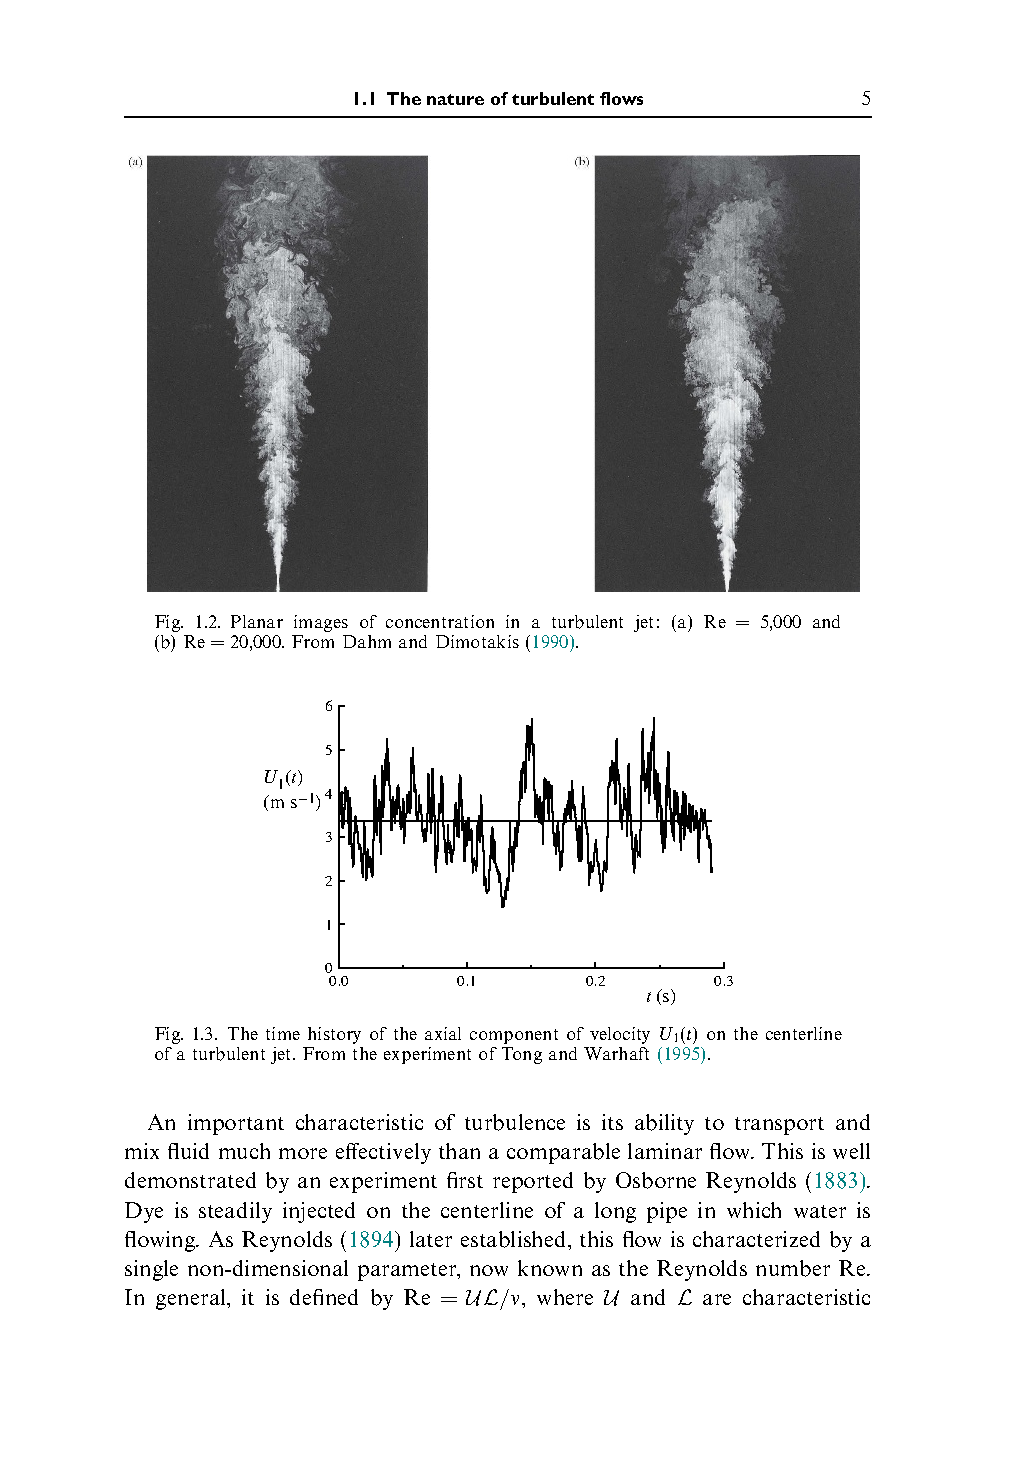
\includegraphics[width=0.8\linewidth,trim={4.3cm 7.7cm 4cm 11.5cm},clip]{Imagenes/03/turbulent}
	\caption{Serie de tiempo para una componente de la velocidad en un flujo turbulento. Fuente: Pope (2000) \cite{pope2000turbulent}.}
	\label{fig:03_turbulent}
\end{figure}

Para entender el origen de la turbulencia, consideremos el número de Reynolds:
\be Re = \frac{LD}{\nu}\ee
el cual se puede interpretar como el cuociente entre las fuerzas inerciales y viscosas en un fluido. Para un fluido que no es turbulento, o sea, laminar, el número de Reynolds es relativamente bajo y eso significa que la viscosidad predomina en su comportamiento. El rol que tiene la viscosidad acá es relevante, ya que es la encargada de atenuar perturbaciones que se puedan dar en las condiciones iniciales o de contorno. A medida que el número de Reynolds crece, la viscosidad irá perdiendo esta capacidad de atenuar las fluctuaciones y se llegará a un punto en donde estas fluctuaciones comenzarán a amplificarse localmente (se alcanza un número de Reynolds crítico y se entra en la zona de transición). A mayor número de Reynolds aún, es inevitable la presencia de inestabilidades en todo el flujo y es acá en donde se alcanza la turbulencia.

Actualmente no existe una definición formal de turbulencia. Luego, en ausencia de esta, se pueden presentar las principales características asociadas a los flujos turbulentos:
\begin{itemize*}
	\item La turbulencia es un proceso aleatorio
	\item La turbulencia contiene un amplio rango de diferentes escalas.
	\item La turbulencia presenta vorticidad aleatoria en pequeñas escalas.
	\item La turbulencia aparece a altos números de Reynolds.
	\item La turbulencia disipa energía.
	\item La turbulencia es un fenómeno del continuo.
	\item La turbulencia es un fenómeno tridimensional.
	\item Las grandes escalas de la turbulencia son insensibles a la viscosidad a altos número de Reynolds.
\end{itemize*}

A continuación se presentan dos de los resultados mas relevantes para el trabajo de tesis, con respecto a la teoría de la turbulencia homogénea e isotrópica.
\subsection{Aleatoriedad y Descomposición de Reynolds}
Reynolds en el año 1894 fue el primero en derivar un conjunto de ecuaciones para flujos turbulentos a través de la reconocida descomposición de Reynolds:
\be u_i = \overline{u}_i + u'_i \ee
Es decir, se descompone el campo de velocidad en una componente media y una componente fluctuante, de esta manera las ecuaciones que se solucionan serán aquellas para el flujo medio evitándose el problema de la aleatoriedad\footnote{El promedio acá se entiende como tanto espacial, temporal o de ensamble; haciendo uso de la teoría ergódica para turbulencia isotrópica homogénea desarrollada.}.

Aplicando esta descomposición junto con propiedades estadísticas del promedio y la conservación de masa, es posible escribir la ecuación de momentum (despreciando las fuerzas de cuerpo) de Navier-Stokes como:
\be\label{eq:03_cons_mom_rans}
(\partial_t \overline{u}_i + \overline{u}_j\partial_j \overline{u}_i)= \nu\partial_{jj}\overline{u}_i -\frac{1}{\rho}\partial_i \overline{p} + \partial_i(\overline{u'_iu'_j})
\ee
Notar que esta estructura es la misma que en la ecuación \ref{eq:cons_mom_nse} salvo que aparece un nuevo término $\overline{u'_iu'_j}$, el cual se le llama \textbf{esfuerzo de Reynolds} y corresponde a la covarianza de las velocidades.

El esfuerzo de Reynolds es el que acarrea la información sobre la turbulencia del flujo y tiene la característica de estar no cerrado, en el sentido que debe modelarse en función de las variables conocidas del problema o resolverla escribiendo una nueva ecuación de transporte para esta (introduciendo nuevas variables no cerradas). En dinámica atmosférica, generalmente la clausura se lleva a cabo utilizando esquemas sencillos que se verán en el próximo capítulo.

Con la introducción del tensor de esfuerzos de Reynolds, se puede definir ahora la energía cinética turbulenta $k$ (en adelante TKE) como:
\be k=\frac{1}{2}\overline{u'_i u'_i} \ee
\subsection{Escalas de la Turbulencia}
Para entender la manera en la que interactúan las distintas escalas presentes en la turbulencia, primero es necesario comprender el concepto de \emph{cascada de energía}. La idea de la cascada de energía fue introducida por Richardson en 1922, expone que la energía cinética entra a la turbulencia en las escalas mas grandes del movimiento. Esta energía es transferida (por un proceso no viscoso) a escalas cada vez mas pequeñas hasta que, en la escala mas pequeña posible, la energía es disipada por los efectos viscosos.

El mecanismo con el cual se lleva a cabo la cascada es la ruptura continua de vórtices. Los vórtices mas grandes son inestables (poseen un $Re$ elevado) y tienden a romperse en vórtices mas pequeños, estos vórtices continúan rompiéndose hasta que el número de Reynolds asociado a los vórtices se hace tan pequeño como para que la viscosidad pueda estabilizar sus estructuras.

La importancia de esta idea radica en que la disipación viscosa ocurre solamente al final de todo el proceso. Esta tasa de disipación $\varepsilon$ debe ser determinada entonces en el inicio de la cascada a través de la transferencia de energía de los vórtices más grandes.

La descripción analítica de las distintas escalas de la turbulencia se hizo por primera vez en 1941 por Kolmogorov a través de la postulación de tres hipótesis:
\paragraph{Hipótesis de Isotropía Local} A un número de Reynolds lo suficientemente elevado, los movimientos turbulentos de las pequeñas escalas son estadísticamente isotrópicos.
\paragraph{Primera Hipótesis de Similaridad} Para cualquier flujo turbulento a un número de Reynolds lo suficientemente elevado, las estadísticas de los movimientos de las pequeñas escalas tienen una forma universal y dependen solamente de $\nu$ y $\epsilon$.

Bajo esta hipótesis, es sencillo demostrar  por análisis dimensional que las pequeñas escalas $\eta$ serán del orden de:
\be \eta \sim \left( \frac{\nu^3}{\varepsilon}\right)^{1/4} \ee
Y su relación con las grandes escalas $l_0$:
\be \frac{\eta}{l_0}\sim Re^{-3/4} \ee
\paragraph{Segunda Hipótesis de Similaridad} Para cualquier flujo turbulento a un número de Reynolds lo suficientemente elevado, las estadísticas de los movimientos de las escalas ubicadas entre $l_0>l>\eta$ tienen una forma universal y dependen únicamente de $\varepsilon$, independiente de $\nu$.

De esta manera, un bosquejo típico log-log de la cascada de energía, se puede ver en la Figura \ref{fig:03_spectra}. Acá se grafica el espectro de energía $E$ en función del número de onda $\kappa$, es decir, cómo se distribuye la energía cinética a través de las distintas escalas espaciales ($\kappa\sim 1/l$).

\begin{figure}[h!]
	\centering
	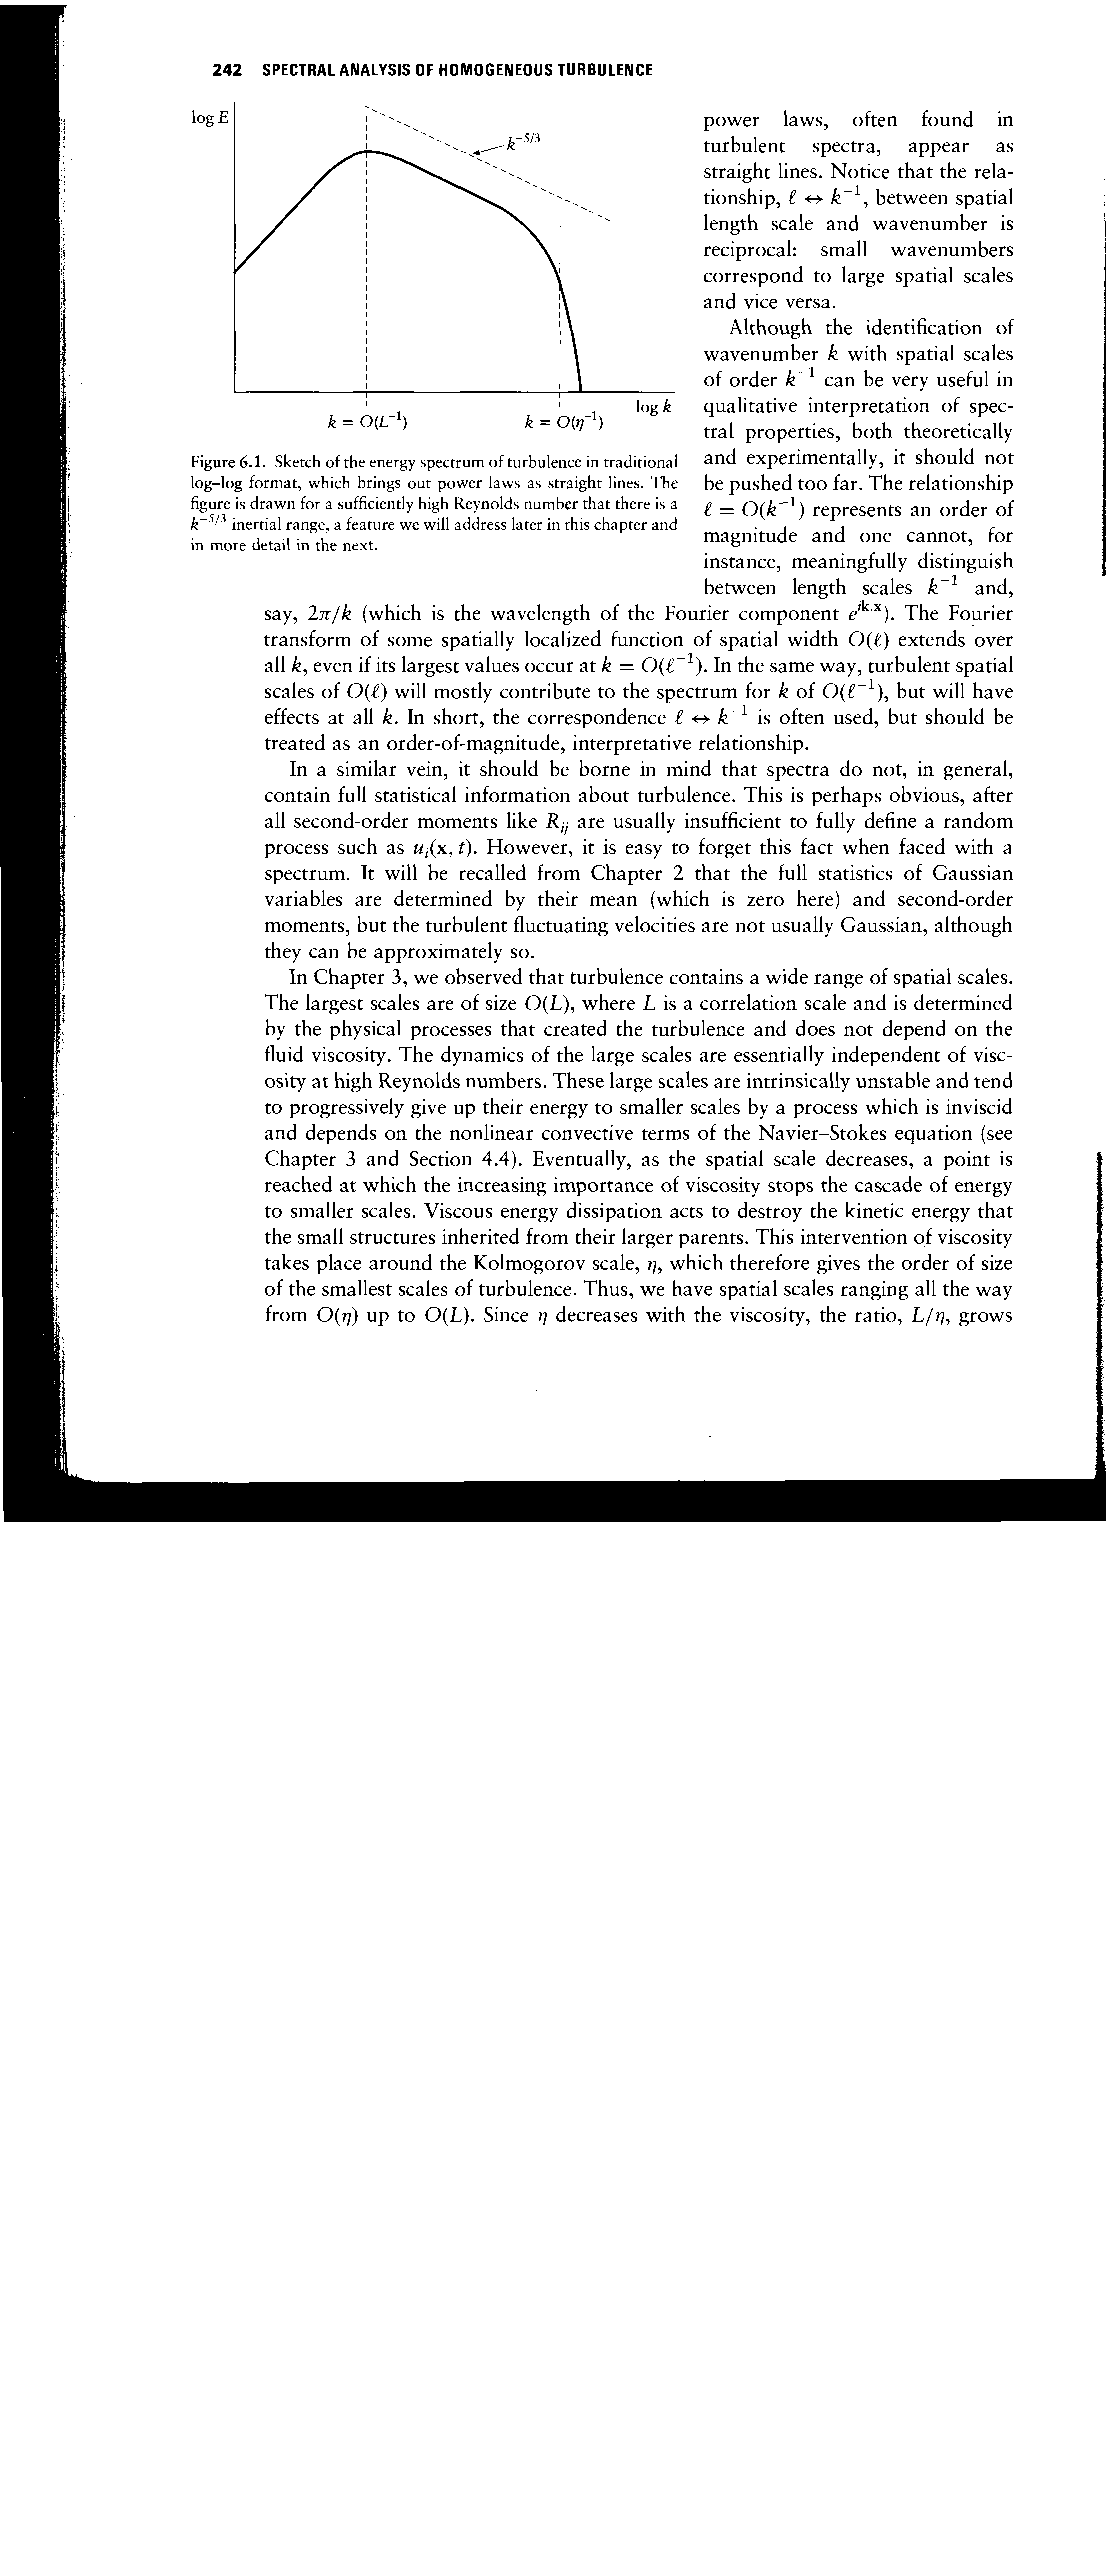
\includegraphics[width=0.85\linewidth,trim={3.2cm 18.3cm 7.0cm 1.5cm},clip]{Imagenes/03/spectra}
	\caption{Gráfico típico log-log de distribución de energía cinética turbulenta con respecto al número de onda $\kappa$ para un flujo con un número de Reynolds elevado. Fuente: Mathieu y Scott (2000) \cite{9780521775380}.}
	\label{fig:03_spectra}
\end{figure}

Tal como se explica anteriormente, existen tres zonas dentro de la cascada de energía. La primera, es la zona de producción de energía cinética asociada a lo grandes vórtices $l_0$. Luego, se ubica el rango inercial, el cual es solo función de la tasa de transferencia de energía y se comporta como una recta. Finalmente, está la microescala o escala de Kolmogorov $\eta$ donde ocurre la disipación.

Con respecto a la escala inercial, se puede demostrar por análisis dimensional que:
\be E(\kappa) = C\varepsilon^{2/3}\kappa^{-5/3} \ee
Este resultado nace de las consideraciones en las hipótesis de Kolmogorov. Se tiene entonces que para turbulencia homogenea e isotrópica, la pendiente (logarítmica) de la energía con respecto al número de onda en la escala inercial es universal y constante, y tiene un valor de -5/3.

De manera operacional, se puede encontrar el espectro de energía turbulenta haciendo una transformada de Fourier del campo de velocidades\footnote{Una definición mas formal del espectro, a través de las funciones de correlación, se puede ver en Mathieu y Scott (2000) \cite{9780521775380}.}. El par que define esta transformada será:
\be \tilde{u}'_i(\vec{\kappa},t) = \frac{1}{(2\pi)^3}\int u'_i(\vec{x},t) e^{-i\vec{\kappa}\cdot\vec{x}}d^3\vec{x} \ee
\be u'_i(\vec{x},t) = \int \tilde{u}'_i(\vec{\kappa},t) e^{-i\vec{\kappa}\cdot\vec{x}}d^3\vec{\kappa} \ee

El espectro de energía cinética turbulenta se puede expresar en función del número de onda $\vec{\kappa}$ como:
\be 
k = \frac{1}{2}\overline{u'_i u'_i} = \int\limits_0^\infty E(\kappa,t)d\kappa
\ee
\be
E(\kappa,t) = 2\pi\kappa^2\phi_{ii}(\kappa,t)
\ee 
\be 
\phi_{ii} \approx \overline{\tilde{u}'_i \tilde{u}'^*_i}
\ee
Acá $E$ es el espectro de energía, $\phi_{ii}$ es la transformada de Fourier de la llamada función de correlación (que en esta formulación funciona como variable auxiliar) y el superíndice $^*$ denota el conjugado.

\newpage 
\section{Fundamentos de Capa Límite Atmosférica}
Se define la capa límite atmosférica (ABL \emph{Atmospheric Boundary Layer} o PBL \emph{Planetary Boundary Layer}) como la parte de la troposfera que está influenciada directamente por la presencia de la superficie terrestre y que responde a las fuerzas superficiales en una escala de tiempo del orden de las horas o menor.

La ABL es altamente variable y se caracteriza por ser turbulenta en la gran mayoría de los casos. Su turbulencia es generada debido al roce con la superficie, la presencia de obstáculos y/o por flotación debido a la temperatura del suelo. 

Existe una estructura bien definida para las capas límites atmosféricas que se desarrollan sobre superficies a alta presión, esta estructura es variable en el tiempo, siendo influenciada principalmente por los ciclos diarios de enfriamiento y calentamiento de la superficie por la radiación solar. En la Figura \ref{fig:03_abl}\footnote{\url{https://commons.wikimedia.org/wiki/File:Atmospheric\_boundary\_layer.svg}} se puede ver la evolución de la estructura de la capa límite en las distintas horas del día (para un día estándar) y sus principales componentes.

\begin{figure}[h!]
	\centering
	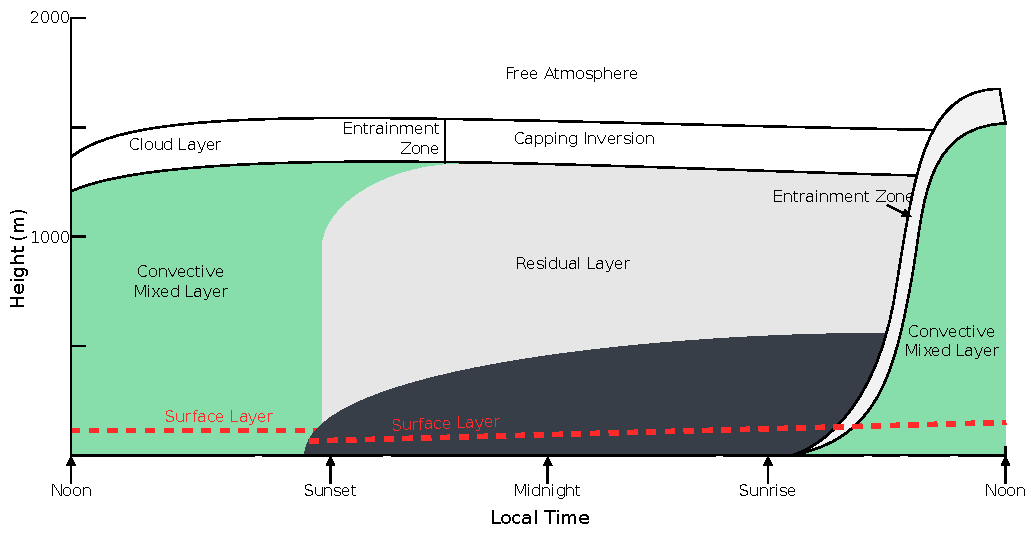
\includegraphics[width=0.98\linewidth,trim={0cm 0cm 0cm 0cm},clip]{Imagenes/03/abl}
	\caption{Evolución diurna de la estructura de la capa límite. Fuente: Wikimedia.}
	\label{fig:03_abl}
\end{figure}

Como se puede ver, la ABL posee 3 grandes componentes: (a) la capa de mezcla o \emph{mixed layer} (b) la capa residual o \emph{residual layer} y (c) la capa límite estable o \emph{stable boundary layer} (en negro). Además de estas, se reconoce la capa de superficie o \emph{surface layer} que es la región al fondo de la capa límite donde los esfuerzos turbulentos no varían mas de un 10\% de su magnitud y que es dominada principalmente por el roce con el terreno. Así, sea cual sea la estructura de la capa límite, el 10\% mas cercano a la superficie va a corresponder siempre a la capa superficial. Finalmente, una capa delgada llamada microcapa o capa de interfaz se ubica en los primeros centímetros de la capa de aire. En esta, el transporte molecular (viscosidad) predomina sobre el transporte turbulento.

Algunas características esenciales de la ABL se mencionan a continuación:
\begin{itemize*}
	\item La humanidad gasta la mayoría de su vida dentro de la ABL.
	\item Los pronósticos del clima son en verdad pronósticos de la capa límite.
	\item La polución queda atrapada en la ABL.
	\item La neblina es creada en la ABL.
	\item La fuente principal de energía para toda la atmósfera es la radiación solar, la cual, en su mayoría es absorbida por el suelo y transmitida al resto de la atmósfera por los procesos de capa límite.
	\item Cerca de un 50\% de la energía cinética de la atmósfera es disipada en la capa límite.
	\item El transporte turbulento de momemtum desde la capa límite a la superficie es el sumidero mas grande de momemtum de la atmósfera.
	\item Las turbinas eólicas extraen energía de los vientos de la ABL.
\end{itemize*}
\subsection{Estructuras de Capa Límite}
\subsubsection{Capa de Mezcla}
Se caracteriza por poseer una turbulencia que usualmente es provocada por la convección, aunque es posible que se forme una especie de capa de mezcla en zonas con vientos fuertes. Las fuentes de convección incluyen la transferencia de calor desde la superficie caliente y el enfriamiento por radiación desde la parte superior de una capa de nubes. La primera de estas, crea movimientos de aire caliente ascendentes desde la superficie de la tierra, mientras que la segunda, genera movimientos descendentes de aire frío desde las nubes. Ambos puedes ocurrir simultáneamente.

En días despejados, el crecimiento de la capa de mezcla está unido al calentamiento solar de la superficie. Comenzando aproximadamente media hora después del amanecer, la altura de la capa de mezcla turbulenta empieza a crecer. La característica fundamental de la capa de mezcla es la mezcla intensa de las variable atmosféricas dentro de esta debido a su condición de ser estáticamente inestable a causa del ascenso de aire caliente. La capa de mezcla alcanza su máxima altura después del mediodía.

Los perfiles de temperatura potencial virtual para esta capa suelen ser generalmente adiabáticos debido a la mezcla, mientras que en la capa superficial es normal hallar perfiles superadiabáticos debido a la superficie caliente.

Sobre la capa de mezcla, una capa estable actua como cubierta de los movimientos ascendentes de aire caliente restringiendo el dominio de la turbulencia. Es la llamada capa de arrastre o \emph{entrainment zone}. Generalmente esta capa es lo suficientemente estable como para que ocurra una inversión térmica y por lo tanto, también se le denomina como capa de inversión.

La rapidez de los vientos dentro de esta capa son subgeostróficos. La parte media de la capa de mezcla presenta un perfil de velocidad que es casi constante (debido a la alta mezcla de momemtum) y un perfil logarítmico en los dominios de la capa de superficie.

\subsubsection{Capa Residual}
En ausencia de advección de aire frío, aproximadamente media hora antes del atardecer, las corrientes ascendentes calientes dejan de existir y la turbulencia en la capa de mezcla decae. La capa de aire que queda se le llama capa residual. Esta capa es de estratificación neutra, lo que implica que la turbulencia es casi de la misma magnitud en todas las direcciones y su perfil de $\theta_v$ es casi adiabático.

Los escalares pasivos que flotaron gracias a la radiación del día se mantendrán en el aire en la capa residual y en el amanecer, cuando la capa de mezcla comienza a arrastrarse con la capa residual, la radiación solar puede provocar reacciones fotoquímicas sobre estos escalares. Esto tiene especial importancia para el caso de la humedad (que se puede considerar a grandes rasgos como un escalar pasivo). En la capa de mezcla la humedad se evapora y quedará retenida dentro de la capa residual, con el pasar de los días, la unificación de la capa residual con la capa de mezcla puede generar formación de nubes en zonas donde, de otra manera, no se podría.

La capa residual no tiene contacto directo con la superficie. Durante la noche, la capa estable aumenta su espesor modificando el fondo de la capa residual. Luego, la capa residual no es afectada por el transporte turbulento de propiedades relacionadas a la superficie y por lo tanto no cae dentro de la definición de lo que se define como capa límite, sin embargo es una estructura dominante de la atmósfera.
\subsubsection{Capa Límite Estable}
A medida que la noche progresa, la parte inferior de la capa residual se transforma debido al contacto con la superficie en una capa límite estable. Esta se caracteriza por ser estáticamente estable y poseer de manera esporádica turbulencia de baja intensidad. Si bien los vientos a nivel de superficie se vuelven mas tranquilos, por sobre esto, el viento puede acelerar a velocidades supergeostróficas en un fenómeno llamado jet nocturno o corriente en chorro de bajo nivel.

Mientras que el aire estáticamente estable tiende a suprimir la producción de turbulencia a nivel de superficie, el desarrollo del jet nocturno fomenta el cortante en el viento, lo cual incita la turbulencia lejos de la superficie. Como resultado, existe turbulencia que se manifiesta en ráfagas cortas que generan mezcla a lo largo de la capa límite estable. Durante los periodos no turbulentos, el movimiento del viento se desacopla de la superficie.

El límite superior de la capa límite estable no es fácilmente identificable como lo es en la capa de mezcla, ya que esta se une suavemente a la capa residual. El largo de la capa estable será la altura en donde la turbulencia es solo una pequeña fracción de su valor superficial.

La velocidad del viento en la noche tiene un comportamiento complejo. En las cercanias de la superficie generalmente se tiene un viento leve o incluso calmado. Sobre los 200 [m] el aire puede alcanzar velocidades de entre 10 a 30 [m/s] en el jet nocturno. Unos cuantos cientos de metros mas arriba y la velocidad del viento disminuye, recuperando su valor geostrófico.

Esta capa estable también es posible que se forme en el día siempre y cuando la superficie sea mas fría que el aire que lo rodea, como puede ser el caso de frentes cálidos o zonas cercanas a la costa.
\subsubsection{Evolución de la Temperatura Potencial}
En la Figura \ref{fig:03_pbl2} se muestra la evolución para la temperatura potencial virtual $\theta_v$ a lo largo de un día estándar. Se puede observar que el perfil de $\theta_v$ da la información suficiente para reconocer perfectamente la estructura de la capa límite. 
\begin{figure}[h!]
	\centering
	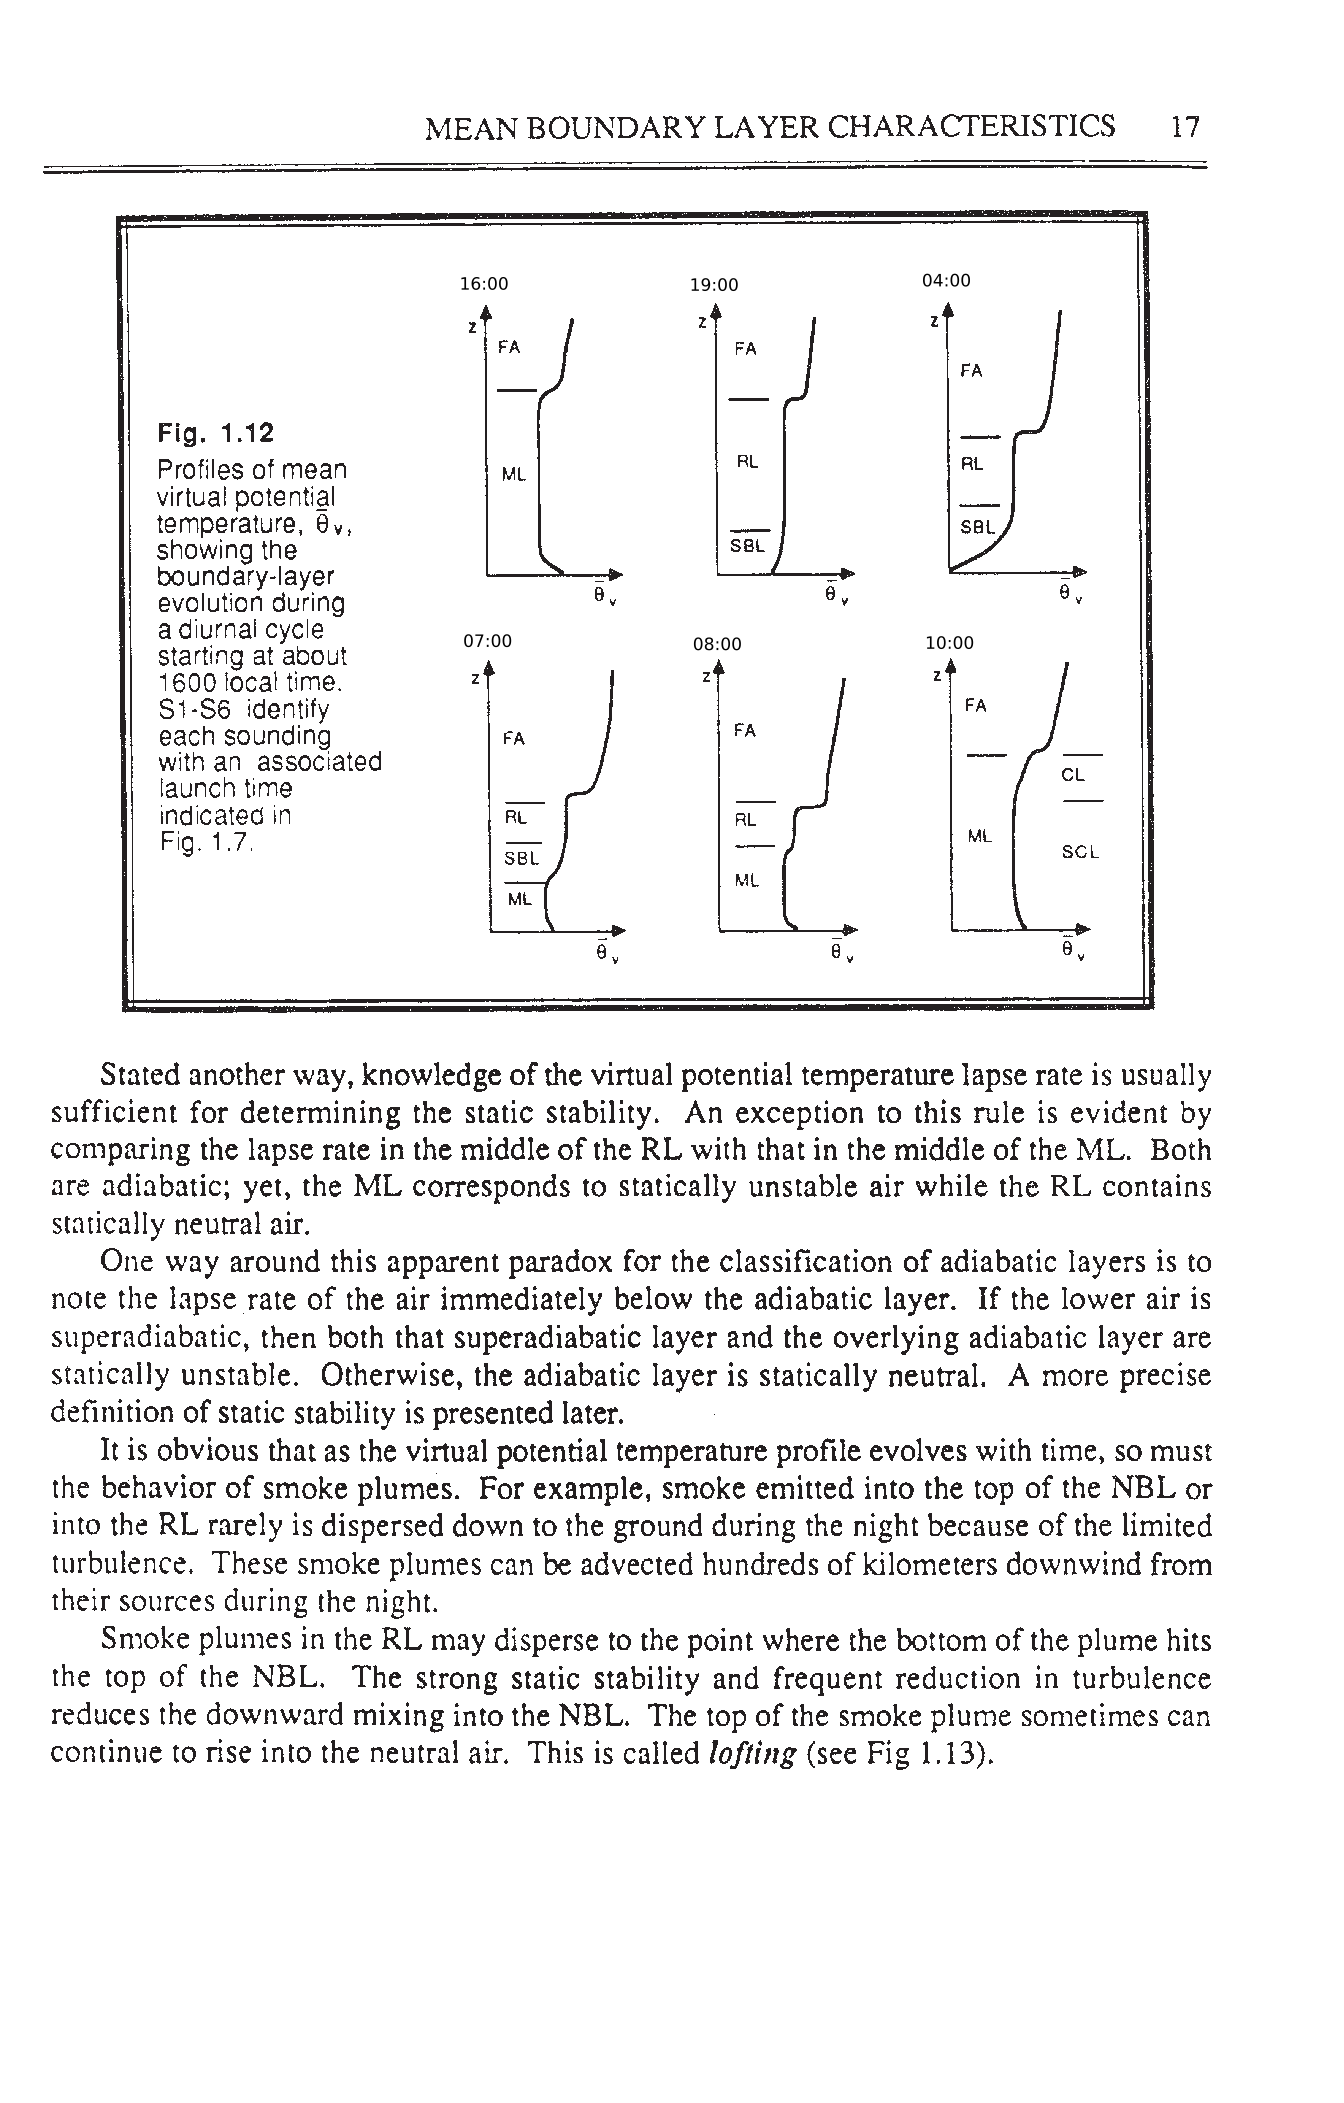
\includegraphics[width=0.7\linewidth,trim={5.6cm 14cm 2.7cm 3.3cm},clip]{Imagenes/03/pbl2}
	\caption{Evolución del perfil de $\theta_v$ en el ciclo diurno. Fuente: Stull (1988) \cite{stull1988introduction}.}
	\label{fig:03_pbl2}
\end{figure}

En esta figura se usan los siguientes acrónimos:
\begin{itemize*}
	\item FA: \emph{Free Atmoshere}, atmósfera libre.
	\item ML: \emph{Mixed Layer}, capa de mezcla.
	\item RL: \emph{Residual Layer}, capa residual.
	\item SBL: \emph{Stable Boundary Layer}, capa límite estable.
	\item CL: \emph{Cloud Layer}, capa de nubes.
	\item SCL: \emph{Subcloud Layer}, capa de subnubes.
\end{itemize*}
\subsection{Esfuerzos Turbulentos}
La turbulencia mezcla momemtum, energía, humedad y contaminantes vertical y horizontalmente. El grado de turbulencia puede ser cuantificado en un término de flujo turbulento (tal como se detalló en la sección anterior). Para el caso del momemtum horizontal, el flujo turbulento vertical será una función de $\overline{w'u'}$ y $\overline{w'v'}$, que son los flujos turbulentos cinemáticos verticales medios.

Los flujos turbulentos cinemáticos medios son negativamente proporcional a los esfuerzos de Reynolds. Este esfuerzo hará que una parcela de aire sufra una deformación. Consideremos el caso vertical en dirección $x$: la velocidad $w'$ generará mezcla de la velocidad $u'$ . La mezcla vertical de $u'$ producirá un esfuerzo en la dirección $x$ y normal a $z$. Este esfuerzo se calcula como:
\be 
\tau_{R,xz} = - \rho \overline{w'u'}
\ee
Ahora, generalmente se quiere saber el esfuerzo total generado por el movimiento horizontal, el cual es relevante a bajas alturas. Se puede demostrar que se puede escribir el flujo turbulento vertical de momemtum horizontal como:
\be 
|\tau_{R,z}| = \rho[(\overline{w'u'})^2 + (\overline{w'v'})^2]^{1/2}
\ee
Coloquialmente a $\tau_{R,z}$ se le conoce también $\tau_{13}$ en la literatura, referenciando a $1$ como la dirección horizontal del viento y $3$ la dirección vertical.

De la misma manera, los flujos turbulentos verticales causan mezcla turbulenta de calor y de humedad desde la superficie. Se pueden anotar estos como:
\be H_f = \rho C_{p,d} (\overline{w'\theta_v'})_s \ee
\be Q_f = \rho (\overline{w'q_v'})_s \ee
\subsubsection{Velocidad de Fricción}
En el contexto de la parametrización de los esfuerzos turbulentos de la superficie, es conveniente introducir una nueva variable de escalamiento para la velocidad que permita reducir el problema. Esta es la llamada velocidad de fricción. Se calcula como:
\be u_* = \sqrt{\frac{|\tau_{R,z}|}{\rho}} \ee
$u_*$ es una métrica de la turbulencia producida mecánicamente debido al roce, al cortante y a la presencia de protuberancias en el terreno.
\subsubsection{Clausura de la Difusión Turbulenta}
La formulación de ecuaciones de transporte para los flujos turbulentos introduce mas incógnitas que ecuaciones. Es necesario entonces, buscar una manera de lograr la clausura del problema introduciendo alguna relación adecuada. Para los flujos en la capa superficial, sea de momemtum, calor, humedad, etc., estos suelen ser estimados mediante la aplicación de: (a) fórmulas para el arrastre aerodinámico (orden 0), (b) teoría de similaridad de Monin-Obukhov (orden 0), (c) teoría del transporte gradiente (orden 1) o (d) teorías con formulaciones de orden superior.

En la formulación de arrastre se tiene:
\be 
(\overline{w'u'})_s = -C_D|\overline{V}_h(z_r)|[\overline{u}(z_r) - \overline{u}(z_{0,m})]
\ee 
$z_{0,m}$ es el largo de rugosidad para la similaridad de momemtum. Notar que $\overline{u}(z_{0,m}) = 0$ por definición. $z_r$ es una altura de referencia (generalmente 10 [m]) y $C_D$ es el coeficiente de arrastre a la altura de referencia.

En la formulación de transporte gradiente se tiene un coeficiente de difusión turbulento de la forma:
\be 
K_{m,zx} = -\frac{(\overline{w'u'})_s}{\partial \overline{u}/\partial z } = C_D |\overline{V}_h(z_r)|(z_r - z_{0,m})
\ee 

Las teorías de arrastre aerodinámico y de transporte gradiente son bien conocidas en el área de la mecánica de fluidos y por lo tanto no trae mayor beneficio el detallarlas acá. Por otro lado, la teoría de similaridad de Monin-Obukhov presenta una mayor intuición acerca del comportamiento de la capa límite y es relevante presentar sus fundamentos, ya que en base a esta se desarrollan la mayoría de los solvers atmosféricos.

\subsubsection{Teoría de Similaridad de Monin-Obukhov}
Se habla de teoría de Monin-Obukhov al referirse a la aplicación de la teoría de similaridad (grupos adimensionales) a la capa límite atmosférica considerando tantos los efectos de roce, como los efectos de flotación.

Una primera relación adimensional que nace de este acercamiento es el gradiente de viento adimensional:
\be \label{eq:03_simi_u}
\frac{\phi_m}{\kappa} = \frac{z}{u_*}\frac{\partial |V_h|}{\partial z}
\ee
Donde $\phi_m$ es un valor que se calcula en función de $z/L$, siendo $L$ es el largo de Monin-Obukhov. $\kappa$ es la constante de Von Karman (usualmente 0,4). Businger et al. (1971) presenta la función de $\phi_m$ de la forma:

\be 
\phi_m = \begin{cases}
	1+\beta_m \frac{z}{L} & \frac{z}{L}>0  \quad\text{estable}\\
	(1-\gamma_m \frac{z}{L})^{-1/4} & \frac{z}{L}<0 \quad \text{inestable}\\
	1 & \frac{z}{L}=0  \quad \text{neutral}
\end{cases}
\ee 
Acá $\beta_m$ y $\gamma_m$ son constantes en función del valor de $\kappa$ que se use \cite{jacobson2005fundamentals}.

El largo de Monin-Obukhov $L$ es una altura proporcional a la altura a la cual la producción de turbulencia debido a la flotación comienza a dominar por sobre la producción debido a efectos mecánicos. Matemáticamente,
\be 
L = \frac{u_*^3\overline{\theta}_v}{\kappa g (\overline{w'\theta'_v})_s} = \frac{u_*^2 \overline{\theta}_v}{\kappa g \theta_*}
\ee 
La segunda igualdad es obtenida sustituyendo por la siguiente relación de similaridad,
\be 
(\overline{w'\theta'_v})_s \approx -u_* \theta_*
\ee
Acá se introduce $\theta_*$ que es una variable de escalamiento para la temperatura potencial\footnote{Se omitirá la manera de aproximar $\theta_*$ en este documento, sin embargo se motiva al lector a leer la referencia \cite{jacobson2005fundamentals} si desea conocer mas al respecto.}. $\theta_*$ es proporcional a la diferencia vertical de temperatura potencial. A mayor valor de $\overline{\theta}$ en la cercanía de la superficie, más negativo será el cambio de temperatura potencial con respecto a la altura y por ende mas inestable será la atmósfera. Para este caso $L$ será negativo pero de un valor pequeño (es inversamente proporcional a $\theta_*$). Si $L$ es pequeño y negativo, $z/L$ es negativo y grande. Estos valores de $z/L$ corresponden a atmósferas inestables debido a la flotación. Análogamente, valores positivos de $z/L$ corresponden a atmósferas estables.

Evidentemente, la introducción de $\theta_*$ permite escribir relaciones de similaridad para el perfil de $\theta$ de la forma:
\be \label{eq:03_simi_theta}
\frac{\phi_h}{\kappa} = \frac{z}{\theta_*}\frac{\partial \overline{\theta}_v}{\partial z}
\ee

\be 
\phi_h = \begin{cases}
	\text{Pr}_t+\beta_h \frac{z}{L} & \frac{z}{L}>0  \quad\text{estable}\\
	\text{Pr}_t(1-\gamma_h \frac{z}{L})^{-1/2} & \frac{z}{L}<0 \quad \text{inestable}\\
	\text{Pr}_t & \frac{z}{L}=0  \quad \text{neutral}
\end{cases}
\ee
Pr$_t$ es el número de Prandtl turbulento, calculado como la razón entre los coeficientes de difusión turbulentos de momemtum $K_m$ y de energía $K_h$ . Para $\kappa=0.4$ se estima un valor de Pr$_t\approx 0.95$.

Todo este desarrollo permite escribir los coeficientes de difusión turbulenta en función de la teoría de similaridad como,
\be 
K_{m,zx} = \frac{\kappa z u_*}{\phi_m}
\ee 
\be 
K_{h,zx} = \frac{\kappa z u_*}{\phi_h}
\ee 

Finalmente, utilizando la teoría de similaridad es posible derivar los perfiles verticales de viento y temperatura potencial virtual (humedad también, pero se ha omitido en este desarrollo). Integrando las ecuaciones \ref{eq:03_simi_u} y \ref{eq:03_simi_theta} se tiene que:
\be 
|\overline{V}_h(z)| = \frac{u_*}{\kappa} \left[ \ln\left( \frac{z}{z_{0,m}} - \psi_m \right) \right]
\ee
\be 
\overline{\theta}_v(z) = \overline{\theta}_v(z_{0,h}) + \text{Pr}_t \frac{\theta_*}{\kappa} \left[ \ln\left( \frac{z}{z_{0,h}} - \psi_h \right) \right]
\ee
Donde:
\be 
\psi_m = \int\limits_{z_{0,m}}^{z}  (1-\phi_m)\frac{dz}{z}\quad;\quad \psi_h = \int\limits_{z_{0,m}}^{z}  (1-\phi_h)\frac{dz}{z}
\ee
Son las funciones de influencia para momemtum y energía que permiten adecuar el perfil logaritmico según la estratrificación. 

Para condiciones neutras se tiene que $\phi_m = 1$ y el perfil de viento horizontal se reduce a su forma:
\be 
|\overline{V}_h(z)| = \frac{u_*}{\kappa} \ln \frac{z}{z_{0,m}}
\ee
la cual es una fórmula clásica para estimar la velocidad del viento dentro de la capa límite.
\subsection{Ecuación de Energía Cinética Turbulenta}
La ecuación de transporte que rige el comportamiento del TKE se puede escribir de la siguiente forma \cite{stull1988introduction}:
\be
\partial_t k + \overline{u}_j\partial_j k = \delta_{i3}\frac{g}{\overline{\theta}_v}\overline{u'_i\theta'_v} - \overline{u'_i u'_j} \partial_j \overline{u_i} - \partial_j\overline{u'_j k} - \frac{1}{\rho} \partial_i \overline{u'_i p'} - \varepsilon
\ee
Donde $\varepsilon$ es la disipación viscosa de energía cinética turbulenta:
\be  \varepsilon = \nu(\overline{\partial_j u'_i\partial_j u'_i}) \ee

Para ganar intuición acerca de los distintos términos presentes en la ecuación, es conveniente tomar un sistema coordenado alineado con la dirección del viento medio y asumir homogeneidad horizontal, además se desprecia la advección relacionada a la componente vertical. De esta manera una forma especial del balance de TKE se puede escribir como:
\newpage
\be
\partial_t k  = \frac{g}{\overline{\theta}_v}\overline{w'\theta'_v} - \overline{u' w'} \partial_z \overline{u} - \partial_z\overline{w' k} - \frac{1}{\rho} \partial_z \overline{w' p'} - \varepsilon
\ee
\vspace{-7mm}
\begin{equation*}
\quad I \quad\qquad II\quad\qquad III\qquad\qquad IV\quad\qquad V\quad\qquad VI
\end{equation*}
El significado físico de cada término es:
\begin{enumerate*}
	\item[I.] Acumulación local o tendencia de TKE.
	\item[II.] Producción o consumo debido a flotación.
	\item[III.] Producción mecánica por cortante.
	\item[IV.] Transporte turbulento de TKE.
	\item[V.] Correlación de presión, describe la distribución de TKE debido a perturbaciones de presión (por flotación o ondas de gravedad).
	\item[VI.] Disipación de TKE.
\end{enumerate*}

Como síntesis, la turbulencia es disipativa. El término $VI$ existe siempre que el TKE no sea cero. Físicamente, esto significa que la turbulencia tiende a decaer y desaparecer a través del tiempo, a no ser que sea creada localmente o trasportada por el flujo medio o procesos turbulentos o de presión. Luego, el TKE no es una cantidad que se conserva. La capa límite puede ser turbulenta solo si existen ciertos procesos físicos generando esta turbulencia.

Las Figuras \ref{fig:03_tke3}, \ref{fig:03_tke1} y \ref{fig:03_tke2} (Fuente: Stull, 1998 \cite{stull1988introduction}) representan la distribución de TKE y el balance de los términos de la ecuación de TKE\footnote{Acá se utiliza una nueva variable de escalamiento $w_*$. Corresponde a una velocidad de escalamiento convectiva. Se calcula como: $[(g\delta/\overline{\theta}_v)(\overline{w'\theta'_v})_s]^{1/3}$.} para distintas horas de un día según simulaciones de varios autores. Estos gráficos y valores servirán de referencia a los valores obtenidos en los resultados de los experimentos de esta tesis.

\begin{figure}[h!]
	\centering
		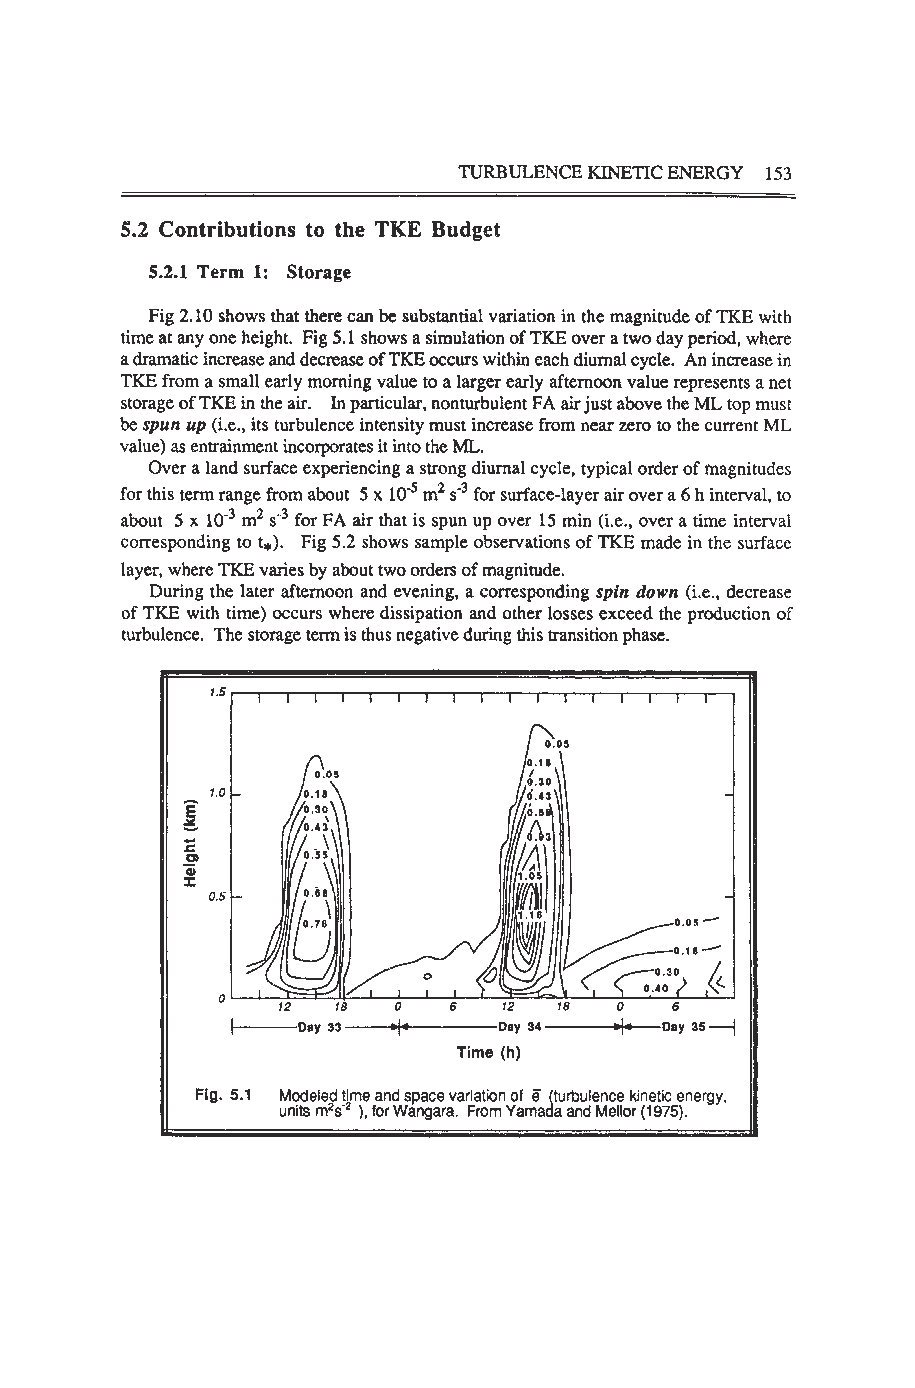
\includegraphics[width=0.8\linewidth,trim={3cm 5.5cm 2.9cm 11.6cm},clip]{Imagenes/03/tke3}
	\caption{Variación espacial y temporal de TKE modelada. Fuente: Stull (1988) \cite{stull1988introduction}.}
	\label{fig:03_tke3}
\end{figure}

La Figura \ref{fig:03_tke3} muestra como el valor del TKE es alto a nivel de superficie y tiende a decaer con la altura. En atmósferas inestables, como lo es a mitad del día, el perfil crece y se obtienen grandes valores para el TKE. Las Figuras \ref{fig:03_tke1} y \ref{fig:03_tke2} muestran como en el día la generación de TKE está dominada por los efectos de flotación y de corte en las zonas muy cercanas a la superficie, y en la noche, estos mecanismos se calman dando espacio a que la disipación actue como sumidero de TKE. Notar el cortante que se genera lejos de la superficie debido al jet nocturno.

\begin{figure}[h!]
	\centering
	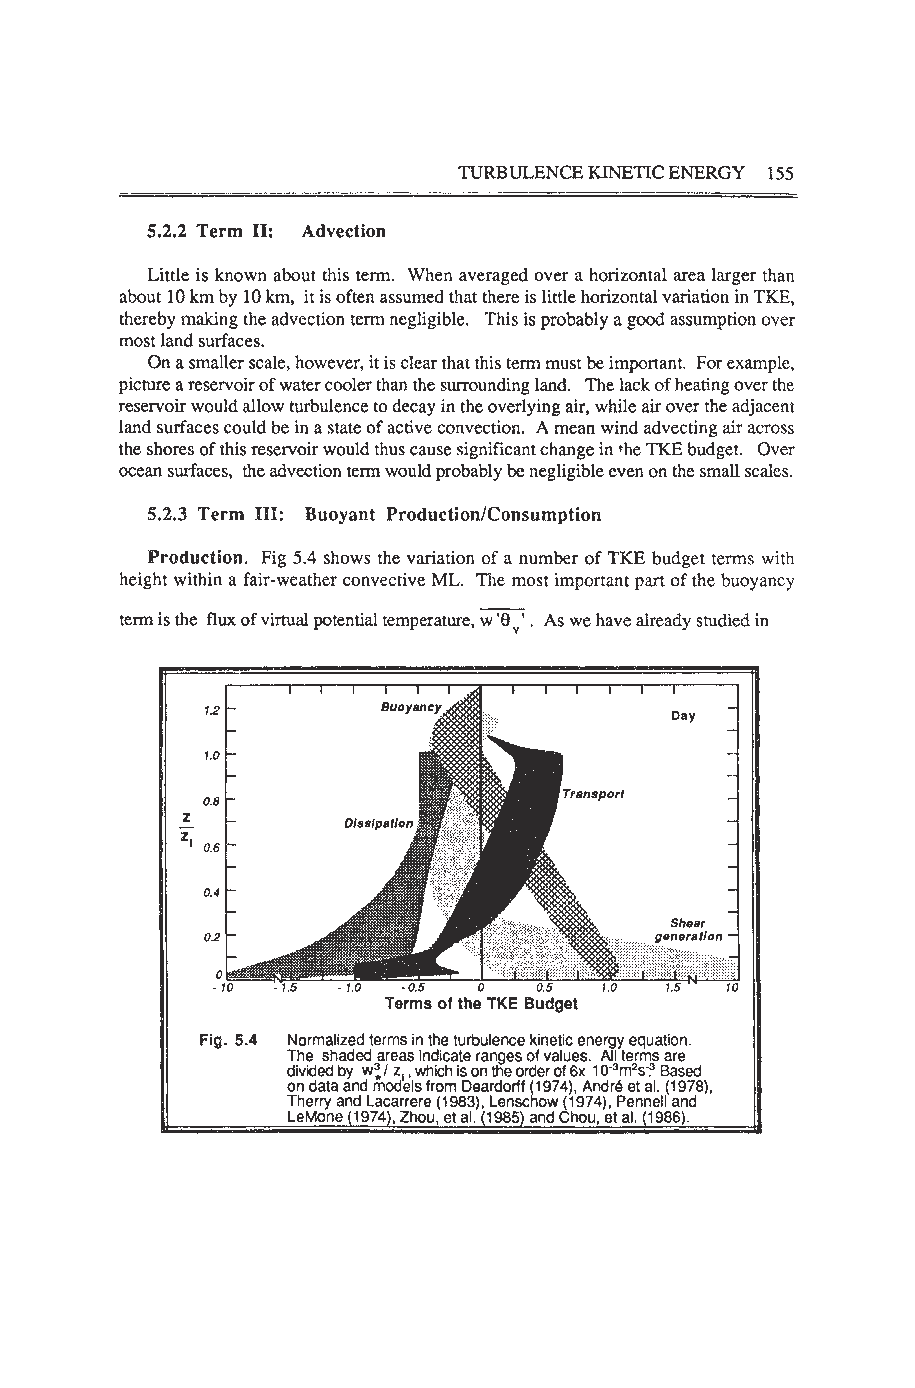
\includegraphics[width=0.8\linewidth,trim={3cm 6.3cm 2.9cm 11.5cm},clip]{Imagenes/03/tke1}
	\caption{Términos normalizados en la ecuación de TKE para el día. Las áreas sombreadas corresponden a un rango de valores. Todos los términos son adimensionalizados por $w_*^3/\delta$. Fuente: Stull (1988) \cite{stull1988introduction}.}
	\label{fig:03_tke1}
\end{figure}

\begin{figure}[h!]
	\centering
		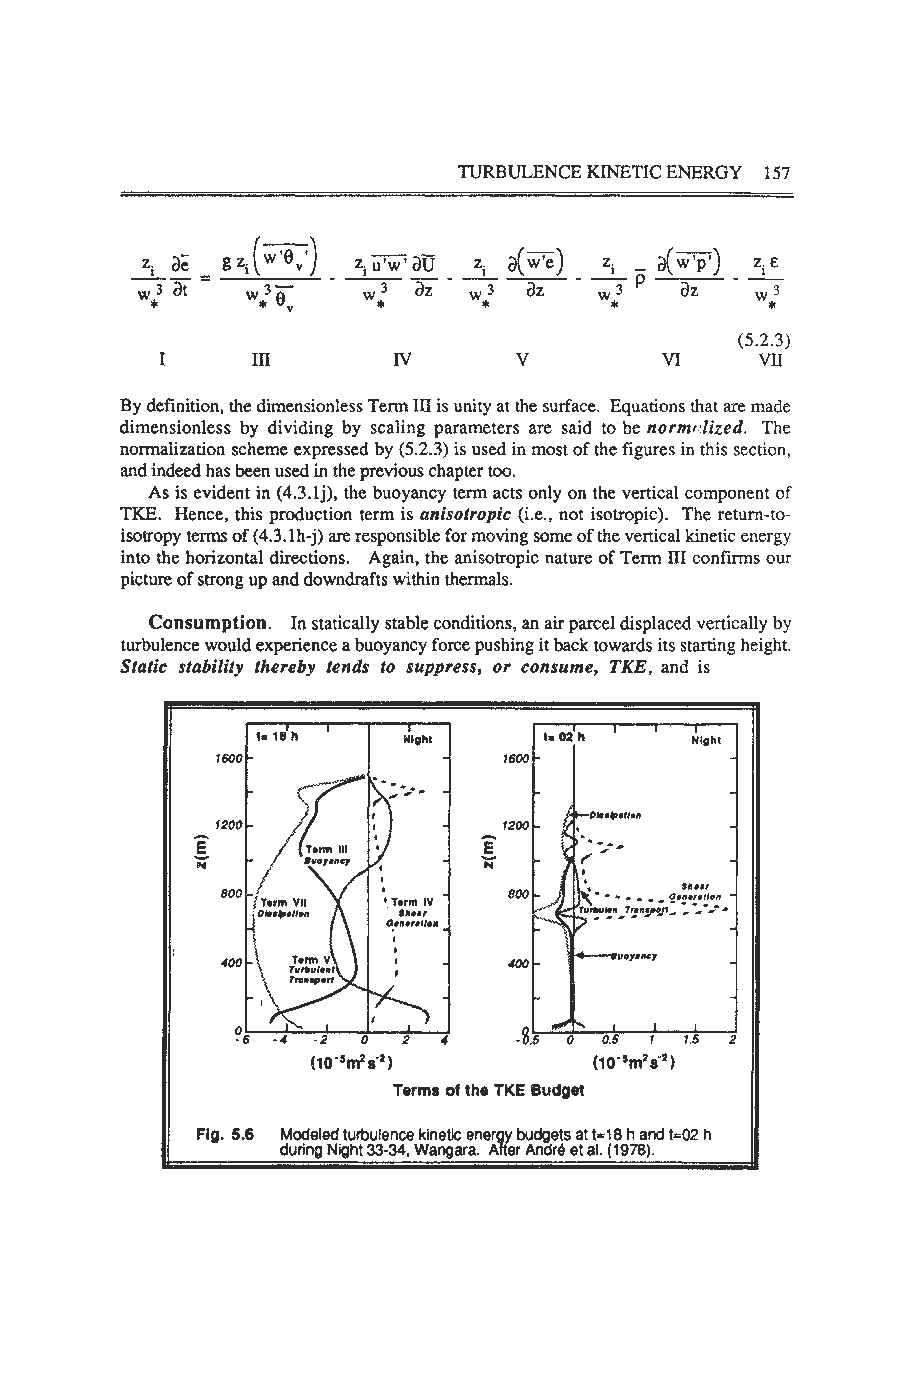
\includegraphics[width=0.8\linewidth,trim={3.2cm 4.8cm 2.8cm 12.1cm},clip]{Imagenes/03/tke2}
	\caption{Términos normalizados en la ecuación de TKE para la noche (18:00 y 02:00). Fuente: Stull (1988) \cite{stull1988introduction}.}
	\label{fig:03_tke2}
\end{figure}
 
Continuando con el análisis de la ecuación de balance de TKE, se introduce ahora un nuevo número adimensional, el \textbf{número de Richardson}, el cual permite revelar la estabilidad del flujo. Se tienen tres formulaciones para este número:

\paragraph{Número de Richardson de Flujo} Corresponde al cuociente entre la producción de TKE por flotación y por efectos mecánicos. Se escribe como:
\be R_f = \frac{(g/\overline{\theta}_v)(\overline{w' \theta'_v})}{(\overline{u'_iu'_j})\partial_j \overline{u}_i} \ee
Es habitual también utilizarlo en su forma simplificada asumiendo homogeneidad horizontal y despreciando la advección vertical como:
\be R_f = \frac{(g/\overline{\theta}_v)(\overline{w' \theta'_v})}{(\overline{u'w'})\partial_z \overline{u} + (\overline{v'w'})\partial_z \overline{v}} \ee
Para flujos estables $R_f$ es positivo. Es más, si $R_f < 1$ el flujo es turbulento, mientras que, para $R_f>1$ el flujo se vuelve laminar.
\paragraph{Número de Richardson Gradiente} El $R_f$ permite saber cuando un flujo turbulento puede volverse laminar, pero impide calcular cuando un flujo laminar puede volverse turbulento (debido a que necesita en su cálculo los flujos turbulentos). Usando un razonamiento análogo a la teoría del transporte gradiente se puede escribir el $R_f$ en términos de gradientes del flujo medio como: 
\be\label{eq:03_richardson} Ri = \frac{(g/\overline{\theta}_v)\partial_z\overline{\theta}_v}{(\partial_z \overline{u})^2+(\partial_z \overline{v})^2} \ee
De esta manera se fija un número de Richardson critico $R_c$ ($0,21\sim0,25$) y de término de turbulencia $R_T$ ($\approx1,0$) y así se puede estimar cuando un flujo laminar se vuelve turbulento o cuando un flujo turbulento se vuelve laminar.
\paragraph{Número de Richardson Global} Debido a que en terreno es difícil conocer los gradientes locales necesarios para la ecuación \ref{eq:03_richardson}, estos se pueden aproximar haciendo uso de mediciones discretas como:
\be R_b = \frac{g \Delta \overline{\theta}_v \Delta z}{\overline{\theta}_v[(\Delta u)^2 + (\Delta v)^2 ]} \ee
Acá el subíndice $b$ es de \emph{bulk}. Este es el número mas usado por los meteorólogos y si bien, no sirve para tener un aproximado de la intensidad turbulenta, si funciona para tener una prueba si/no con respecto a la existencia de esta.
\newpage

\section{Large Eddy Simulation}
Hasta ahora, el problema de la turbulencia se ha acotado a separar el flujo en su componente media y sus fluctuaciones, y luego modelar los esfuerzos turbulentos. En esta sección se introducirá una manera alternativa de escribir un campo turbulento como suma de una componente filtrada y otra residual. Como se mencionó en el capítulo 2, estos dos acercamientos van a generar las mismas ecuaciones, sin embargo la diferencia radica en la manera en la que se lleva a cabo la clausura.

Si se considera la naturaleza multiescala de la turbulencia, resulta natural querer resolver los campos de flujo separando las escalas de producción (relacionadas con los grandes vórtices y el ingreso de energía) de las escalas pequeñas (relacionadas a los vórtices en la escala de Kolmogorov y a la disipación de energía). La manera de realizar esto es aplicando un operador de filtro a las variables, de modo que actúe a nivel del espectro de energía, separando las escalas grandes de las pequeñas. De ahí el nombre Simulación de Grandes Vórtices o Large Eddy Simulation (LES) en inglés. 

El desarrollo del LES fue motivado principalmente por aplicaciones meteorológicas (Smagorinsky (1963), Lilly (1967), Deardorff (1974)) y su implementación en la ABL sigue siendo un foco de investigación activo para el LES. 

Formalmente, se pueden considerar cuatro pasos conceptuales para la aplicación del LES:
\begin{enumerate*}
	\item[i.] La operación de filtrado descompone las variables (por ejemplo, la velocidad $u_i(x_i,t)$) en la suma de una componente filtrada (o resuelta) $\overline{u}_i(x_i,t)$, y una componente residual (o de submalla) $u'_i(x_i,t)$. El campo filtrado va a representar el movimiento de los grandes vórtices.
	\item[ii.] Se derivan la ecuaciones de transporte para el campo filtrado a través de las ecuaciones de Navier-Stokes. Estas ecuaciones mantienen su forma estándar con la excepción de la incorporación del tensor de esfuerzos residuales (o de submalla).
	\item[iii.] Se logra la clausura mediante la modelación del tensor de esfuerzo residuales. La manera más sencilla es a través de un modelo de viscosidad turbulenta.
	\item[iv.] Las ecuaciones filtradas son solucionadas numéricamente.
\end{enumerate*}
\subsection{Filtrado}
El operador de filtrado es definido como:
\begin{equation}
\overline{u}(x_i,t) = \int G(r_i,x_j) u(x_j-r_i,t)dr_i
\end{equation}
Donde la integración se realiza en todo el dominio del flujo. Notar que el filtro corresponde a una operación de convolución en el sentido del análisis de Fourier. El kernel $G$ del filtro satisface una condición de normalización:
\begin{equation}
\int G(r_j,x_i)dr_j = 1
\end{equation}
Se define entonces una magnitud residual basada en la operación de filtrado como:
\begin{equation}
u' = u - \overline{u}
\end{equation}
Es decir, se separa la variable de interés en una parte filtrada y su residuo. Está descomposición es, a priori, análoga a una descomposición de Reynolds. Sin embargo, hay dos diferencias importantes: (a) $\overline{u}(x_i,t)$ sigue siendo una variable aleatoria y (b) que, en general, el residuo filtrado no es cero:
\be \overline{u'}(x_i,t) \not= 0 \ee
Estas diferencias se pueden apreciar en la Figura \ref{fig:03_les}.
\begin{figure}[h!]
	\centering
	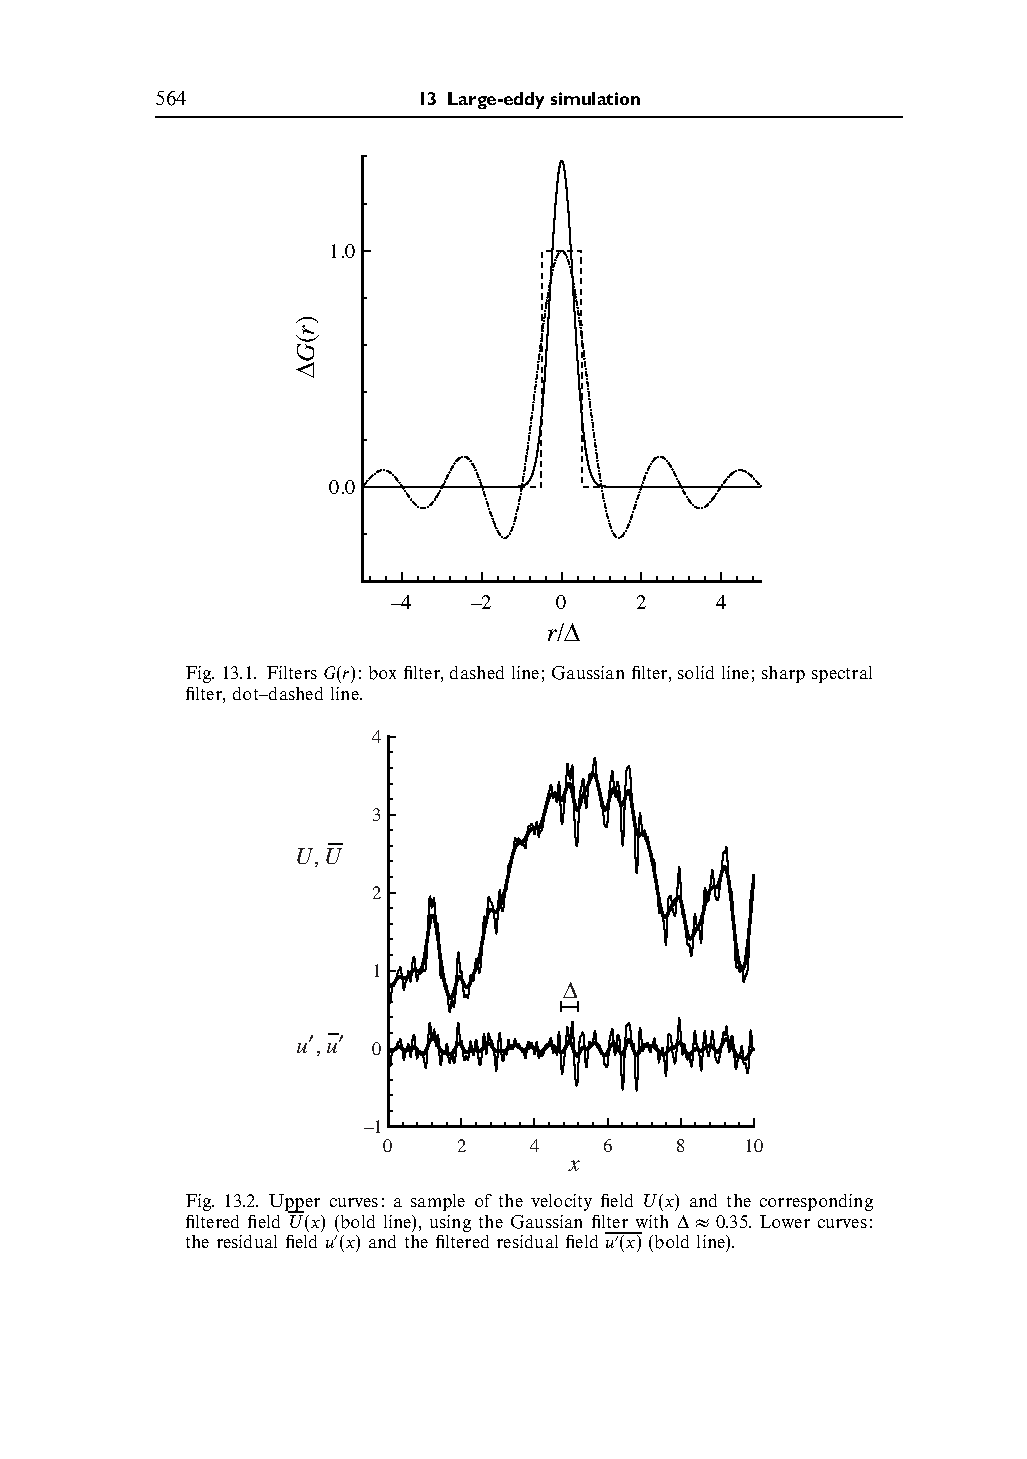
\includegraphics[width=0.6\linewidth,trim={4.8cm 4.8cm 2.8cm 12.1cm},clip]{Imagenes/03/les}
	\caption{Curva superior: una muestra de un campo de velocidad $u$ y su correspondiente campo filtrado $\overline{u}$ (en negrita). Curva inferior: campo residual $u'$ y campo residual filtrado $\overline{u'}$ (en negrita). Fuente: Pope (2000) \cite{pope2000turbulent}.}
	\label{fig:03_les}
\end{figure}

Se debe tener en cuenta que el filtro es en el fondo un nuevo operador matemático que cumple sus propias propiedades y que permite separar las escalas grandes de las pequeñas. Para una mejor descripción teórica de lo que implica un operador de filtrado se puede recurrir a Berselli et al. (2005) \cite{9783540263173}.

\subsection{Ecuaciones de Conservación Filtradas}
La aplicación del filtro a la ecuación de conservación de masa para flujo incompresible, da como resultado el hecho de que tanto el campo filtrado $\overline{u}$ como el campo residual $u'$ son solenoidales,
\be \partial_i \overline{u}_i = \partial_i u'_i = 0\ee
Utilizando esto, se escribe la ecuación de momemtum filtrada como:
\be
\partial_t \overline{u}_i + \partial_j(\overline{u_j u_i}) = \frac{1}{\rho} \partial_i \overline{p} + \nu\partial_{jj}\overline{u}_i
\ee
Se define el tensor de esfuerzos residuales como:
\be \tau_{ij}^R \equiv \overline{u_j u_i} - \overline{u}_j \overline{u}_i \ee
El cual es análogo al tensor de esfuerzos de Reynolds\footnote{Para diferenciar la notación, se utilizan corchetes para indicar promedio y $^*$ para indiciar fluctuaciones. De esta forma la descomposición de Reynolds se escribe $u_i = \langle u_i\rangle + u^*_i$}:
\be \langle u^*_i u^*_j \rangle = \langle u_i u_j \rangle - \langle u_i \rangle \langle u_j \rangle \ee
La energía cinética residual es:
\be k_r = \frac{1}{2}\tau_{ii}^R \ee
Y el tensor de esfuerzos residuales anisotrópicos se define como:
\be \tau_{ij}^r = \tau_{ij}^R - \frac{2}{3}k_r \delta_{ij} \ee
El segundo término de la ecuación anterior corresponde al esfuerzo residual isotrópico. Este se puede incluir dentro de la presión para reescribir la ecuación de momemtum como:
\be
\partial_t \overline{u}_i + \overline{u}_j \partial_j(\overline{u}_i) = \frac{1}{\rho} \partial_i \overline{p} + \nu\partial_{jj}\overline{u}_i - \partial_j \tau_{ij}^r
\ee

Para formar una ecuación de transporte para la energía cinética del campo filtrado primero se aplica el filtro a la energía cinética del campo total $E$ como:
\be \overline{E} = \frac{1}{2}\overline{u_i u_i} \ee
Esta puede ser descompuesta como:
\be \overline{E} = E_f + k_r \ee
donde $E_f=\frac{1}{2}\overline{u}_i\overline{u}_i$ es la energía cinética del campo filtrado y $k_t$ es la energía cinética residual.

Ahora, una contracción de la conservación de momemtum filtrada con $\overline{u}_i$ da la ecuación de transporte para $E_f$:
\be  
\partial_t E_f + \overline{u}_j\partial_j E_f + \frac{1}{\rho}\partial_i(\overline{u}_i\overline{p})+\partial_j(\overline{u}_i\tau_{ij}^r)-2\nu\partial_j(\overline{u}_i\overline{S}_{ij})= - \varepsilon_f -\Pi
\ee
Los términos al lado izquierdo corresponden a términos de transporte. Al lado derecho se ubican las fuentes o sumideros. $\varepsilon_f$ corresponde a la disipación viscosa por el campo de velocidad filtrado:
\be \varepsilon_f = 2\nu \overline{S}_{ij}\overline{S}_{ij} \ee
$\Pi$ es la tasa de producción de energía cinética residual (o disipación de submalla). Representa el traspaso de energía desde las escalas filtradas a las residuales y puede ser positivo o negativo (permitiendo \emph{backscatter}),
\be 
\Pi = -\tau_{ij}^r\overline{S}_{ij}
\ee 
\subsection{Modelación de los Esfuerzos Residuales}
Para lograr la clausura de las ecuaciones filtradas, se necesita un modelo para el esfuerzo residual anisotrópico $\tau_{ij}^r$. El modelo mas simple es el propuesto por Smagorinsky (1963), el cual también sirve como base para varios modelos mas avanzados.
\subsubsection{Modelo de Smagorinsky}
El modelo se puede ver en dos partes. Primero el modelo de viscosidad turbulenta lineal:
\be \tau_{ij}^r = -2\nu_t \overline{S}_{ij} \ee
se usa para relacionar el esfuerzo residual con la tasa de deformación filtrada. El coeficiente de proporcionalidad $\nu_t(x_i,t)$ es la viscosidad turbulenta de los movimientos residuales. 

Segundo, a través de una analogía con la hipótesis de largo de mezcla, la viscosidad turbulenta se modela como:
\be \nu_t = \ell_s^2 \overline{\mathcal{S}} \ee
\be \nu_t = (C_S \Delta)^2 \overline{\mathcal{S}} \ee
donde $\mathcal{S}$ es la tasa de deformación filtrada característica. $\ell_s$ es la escala de longitud de Smagorinsky, la cual, por medio de un coeficiente de Smagorinsky $C_s$($\sim 0,17$) se toma como proporcional al ancho del filtro $\Delta$.
\subsubsection{Modelo de Deardorff}
Tomando en consideración que el modelo de Smagorinsky es instantáneo y local, se torna natural el buscar incorporar los efectos no locales y de historia a través de alguna ecuación de transporte para $\tau_{ij}^r$. 

Deardorff (1974) planteó una ecuación de transporte para $k_r$\footnote{La estructura de la ecuación de transporte puede variar según el caso. Para motivos de esta tesis la forma de esta ecuación se verá en el próximo capítulo.} y logró la clausura a través de las siguientes relaciones:
\be \varepsilon_r = \frac{C_E k_r^{3/2}}{\Delta} \ee
\be \nu_t = C_v k_r^{1/2}\Delta \ee
Donde $C_E\approx 0.7$ y $C_v\approx 0.1$. $\varepsilon_r$ es la tasa de disipación de energía cinética residual. Modelos de este tipo son ampliamente usados en meteorología y es este el que se implementa en las simulaciones de esta tesis.
\newpage
\section{Asimilación de Datos}
La asimilación de datos (\emph{Data Assimilation}, en adelante DA) es un método de análisis con el cual información proveniente de observaciones es incorporado dentro de un modelo de estado. El modelo impone la consistencia dinámica sobre las variables y se encarga de esparcir la información espacialmente y sobre las variables.

Existen tres componentes en un proceso de asimilación de datos: las observaciones; el \emph{background}, que es la información sobre el estado de la atmósfera proveniente de algún modelo u otro análisis; y las restricciones dinámicas, que las impone el modelo.

Sea $\mathbf{x}$\footnote{Para esta sección se utilizará la negrita para indicar vectores y matrices.} el vector de estado de tamaño $n$ que define el estado de la atmósfera basado en algún modelo o análisis\footnote{La dimensión de $\mathbf{x}$ será igual a la cantidad de elementos en la malla multiplicado por la cantidad de variables de estado del modelo.} y sea $\mathbf{x}_t$ el vector que representa la mejor aproximación posible del estado de la atmósfera en la malla numérica\footnote{Notar que $\mathbf{x}_t$ no es el estado real instantáneo de la atmósfera debido a los errores de representación del modelo.}. El vector de \emph{background} $\mathbf{x}_b$, será la primera aproximación para $\mathbf{x}_t$. Si se denomina $\mathbf{x}_a$ al resultado del análisis, el problema se reduce entonces a hallar la corrección $\delta \mathbf{x}$ tal que,
\begin{equation*}
	\mathbf{x}_a = \mathbf{x}_b + \delta \mathbf{x}
\end{equation*}
sea lo mas cercano posible a $\mathbf{x}_t$.

Las observaciones utilizadas en el análisis se almacenan en el vector de observación $\mathbf{y}$. En el proceso de análisis este vector de observación debe ser comparado con un vector de estado. Como cada grado de libertad del vector de estado evidentemente no tendrá su correspondiente observación, es necesario llevar a cabo una transformación desde el espacio del modelo hacia el espacio de observación. Esta transformación se realiza a través del operador de observación $H(\mathbf{x})$\footnote{$H(x)$ es una matriz también, sin embargo, y solo para este caso, no se utiliza la negrita para diferenciarla del operador linealizado $\textbf{H}$ que se verá mas adelante}. Básicamente este operador interpola las variables de estado desde los puntos de la malla numérica a los puntos de observación a través de una interpolación adecuada (por ejemplo: lineal o cuadrática) . La diferencia
\begin{equation*}
	\mathbf{y}-H(\mathbf{x}_b)
\end{equation*}
se llama vector de innovación, y la diferencia
\begin{equation*}
\mathbf{y}-H(\mathbf{x}_a)
\end{equation*}
es el residual del análisis.

Usando esta notación, el problema se puede escribir como:
\begin{equation}\label{eq:03_dataassim1}
	\mathbf{x}_a = \mathbf{x}_b + \mathbf{K}(\mathbf{y} - H(\mathbf{x}_b))
\end{equation}
donde $\mathbf{K}$ es la matriz peso de la innovación que se debe encontrar.
\subsection{Análisis Variacional Tridimensional}

Si bien es posible hallar una solución teórica al problema multidimensional expresado en la ecuación \ref{eq:03_dataassim1}, generalmente es ineficiente y por lo tanto se adopta una metodología de minimización de funcion de costo o, análisis variacional.

Se puede demostrar \cite{warner2010numerical} que el problema variacional multidimensional busca minimizar una función de costo $J(\mathbf{x})$, que pondera los errores provenientes del modelo $J_b$ (\emph{background}) y de las observaciones $J_o$ de la forma:

\be 
J(x) = J_b + J_o = \frac{1}{2}(\textbf{x}-\textbf{x}_b)^T \textbf{B}^{-1}(\textbf{x}-\textbf{x}_b) + \frac{1}{2}(H(\textbf{x})-\textbf{y})^T \textbf{R}^{-1}(H(\textbf{x})-\textbf{y})
\ee 
Acá $\textbf{B}$ es la matriz de covarianzas de los errores del \emph{background} y $\textbf{R}$ es la matriz de covarianzas de los errores de las observaciones. La importancia y desarrollo de estas se explicarán mas adelante.

Teóricamente el problema variacional se soluciona hallando el gradiente de la función de costo e igualando a cero, es decir:
\be 
\nabla J(x) = \textbf{B}^{-1}(\textbf{x}-\textbf{x}_b)-H^T\textbf{R}^{-1}(\textbf{y}-H(\textbf{x}))=0
\ee
Despejando se puede tener una solución analítica de la forma:
\be \label{eq:03_dataassim}
\textbf{x}_a = \textbf{x}_b + \textbf{B}H^T(H\textbf{B}H^T+\textbf{R})^{-1}(\textbf{y}-H(\textbf{x}_b)) 
\ee
La ecuación anterior es fácil de entender si se identifican las matrices $H\textbf{B}H^T$ que es la proyección del error del background en el espacio de observacion y $\textbf{B}H^T$ que es la proyección del error del background en espacio de background-observación. De esta manera el análisis no es mas que una combinación de la ponderación de los errores aplicado al vector de innovación.

Utilizando la terminología de la sección anterior, se deriva que:
\be
\mathbf{K} = \textbf{B}H^{T}(H\textbf{B}H^T + \textbf{R})^{-1}
\ee 
Esta matriz $K$ de peso de la innovación, nuevamente, es computacionalmente intensiva calcularla para un gran número de observaciones, es por esto que en la práctica el problema variacional se resuelve usando algún método de minimización o algoritmo descendiente como el gradiente conjugado o métodos de cuasi-Newton.
\subsection{Matrices de Covarianzas $\textbf{B}$ y $\textbf{R}$}
Las matrices de covarianzas cumplen un rol fundamental en el proceso de análisis, ya que son ellas las que se encargan de ponderar correctamente los valores del \emph{background} y de las observaciones de manera realista. 

La matriz $\textbf{B}$ es la matriz de covarianzas de los errores del \emph{background}, sus dimensiones son de $n\times n$. La correcta estimación de esta matriz es muy importante para el proceso de análisis ya que  controla la influencia para el incremento del análisis en términos de la magnitud y de su forma. Con respecto a la forma, define el esparcimiento de la información desde una observación hasta la malla de análisis, y con respecto a la magnitud, si los errores del \emph{background} son grandes se le da un mayor peso a la observación.

Para un caso multi-dimensional:
\be 
\mathbf{B} = \overline{(\varepsilon_b - \overline{\varepsilon}_b)(\varepsilon_b - \overline{\varepsilon}_b)^T}
\ee 
Donde $\varepsilon$ es el vector de errores.
La matrix $\textbf{B}$ corresponde a una matriz cuadrada y simétrica con variazas a los largo de su diagonal. Por ejemplo, para un caso simple tridimensional:
\be 
\textbf{B} = \begin{pmatrix}
	\text{var}(e_1) & \text{cov}(e_1,e_2) & \text{cov}(e_1,e_3) \\
	\text{cov}(e_1,e_2) & \text{var}(e_2) & \text{cov}(e_2,e_3) \\
	\text{cov}(e_1,e_3) & \text{cov}(e_2,e_3) & \text{var}(e_3) \\
\end{pmatrix}
\ee 
Los términos fuera de la diagonal son las covarianzas cruzadas entre cada par de variables\footnote{Acá variable se usa en el sentido de cada variable dependiente en cada punto de malla} en el modelo. Hay tres maneras para estimar esta matriz:
\begin{enumerate*}
	\item[1.] \textbf{Covarianzas del error precalculadas:} Algunos métodos de asimilación de datos usan covarianzas precalculadas que pueden estar basadas en (a) un promedio de muchos estados distintos de la atmósfera, (b) consideraciones teóricas, o (c) simulaciones numéricas. Este último método es el que aplica el software WRF para hallar $\textbf{B}$.
	\item[2.] \textbf{Ponderación espacial anisotrópica no óptima:} Un ejemplo de esta metodología, por ejemplo, utiliza la información de la orografía para controlar la dispersión del vector de innovación a baja altura. La justificación de esto es que las covarianzas entre puntos que están en lados opuestos a una montaña deben ser pequeñas. De esta manera, la distribución del incremento de análisis es anisotrópica.
	\item[3.] \textbf{Covarianzas del error completamente régimen-dependiente:} Los métodos anteriores no toman en consideración los eventos diarios meteorológicos que se llevan a cabo en la atmósfera y que influyen fuertemente en la manera en la que las observaciones se analizan. Algunos métodos de asimilación de datos sofisticados, calculan las covarianzas del error del \emph{background} en función del flujo que evolucionan a través del proceso de asimilación.
\end{enumerate*}



Con respecto a la matriz $\textbf{R}$, esta es la matriz de convarianzas de los errores de las observaciones, sus dimensiones son de $p\times p$, donde $p$ es la cantidad de observaciones a analizar. Generalmente los errores de las observaciones son considerados independientes, especialmente cuando son realizadas por distintos instrumentos. Las varianzas generalmente son estimadas basadas en el conocimiento de las características de los instrumentos, los cuales pueden ser estudiados en el laboratorio. La mayoría de los modelos de $\textbf{R}$ son diagonales o casi diagonales.